\documentclass[aspectratio=169,11pt,hyperref={colorlinks=true}]{beamer}
% https://github.com/zr-tex8r/BXcjkjatype/blob/master/README-ja.md
\usepackage[whole]{bxcjkjatype}
\usetheme{boxes}
\setbeamertemplate{navigation symbols}{}
\definecolor{openstack}{RGB}{149,0,4}
\setbeamercolor{titlelike}{fg=openstack}
\setbeamercolor{structure}{fg=openstack}
\hypersetup{colorlinks,urlcolor=openstack}
\setbeamertemplate{footline}[frame number]
% Inserting graphics
\usepackage{graphicx}
% Side-by-side figures, etc
\usepackage{subfigure}
% Code snippits
\usepackage{listings}
% Color stuff
\usepackage{color}
% underline
\usepackage{soul}

\usepackage{amsmath}
\usepackage{tikz}
\newcommand\RBox[1]{%
  \tikz\node[draw,rounded corners,align=center,] {#1};%
}
\usepackage{hyperref}
%\usecolortheme{buzz}
%\usecolortheme{wolverine}
%\usetheme{Boadilla}
\usepackage[T1]{fontenc}
%\usepackage{fontspec}
%\setmainsfont{hiragino-elcapitan}
%\usepackage[expert, deluxe]{otf}

\definecolor{mygreen}{rgb}{0,0.6,0}
\definecolor{mygray}{rgb}{0.5,0.5,0.5}
\definecolor{mymauve}{rgb}{0.58,0,0.82}


%\usepackage{CJK}
%\pdfmapline{=genshingothic@Unicode@ <genshingothic.ttf}
% bxcjkjatype
%\setgothicfont[<ID>]{<フォントファイル名>}
%\setgothicfont{/Users/foo/Library/Fonts/genshingothic.ttf}
%\setgothicfont{/Users/foo/Library/Fonts/NotoSansCJKjp-Regular.otf}
%\setgothicfont{/Users/foo/Downloads/genshingothic-20150607/GenShinGothic-P-Normal.ttf}
%\setgothicfont{/Users/foo/Downloads/genshingothic-20150607/GenShinGothic-Regular.ttf}
%\setgothicfont{hiragino.ttc}
\setgothicfont{mplus-1p-regular.ttf}
\setCJKfamilydefault{\gtdefault}
%\setCJKfamilydefault{\mcdefault}
%\CJKforce{abcdefghijklmnopqrstuvwxyzABCDEFGHIJKLMNOPQRSTUVWXYZ}


\lstset{%
  backgroundcolor=\color{white},   % choose the background color; you must add \usepackage{color} or \usepackage{xcolor}
  breakatwhitespace=false,         % sets if automatic breaks should only happen at whitespace
  breaklines=true,                 % sets automatic line breaking
  captionpos=b,                    % sets the caption-position to bottom
  commentstyle=\color{openstack},  % comment style
  extendedchars=true,              % lets you use non-ASCII characters; for 8-bits encodings only, does not work with UTF-8
  keepspaces=true,                 % keeps spaces in text, useful for keeping indentation of code (possibly needs columns=flexible)
  keywordstyle=\color{blue},       % keyword style
%  otherkeywords={*,...},           % if you want to add more keywords to the set
  numbersep=5pt,                   % how far the line-numbers are from the code
  numberstyle=\tiny\color{mygray}, % the style that is used for the line-numbers
  rulecolor=\color{black},         % if not set, the frame-color may be changed on line-breaks within not-black text (e.g. comments (green here))
  showspaces=false,                % show spaces everywhere adding particular underscores; it overrides 'showstringspaces'
  showstringspaces=false,          % underline spaces within strings only
  showtabs=false,                  % show tabs within strings adding particular underscores
  stringstyle=\color{openstack},   % string literal style
}

\setbeamerfont{caption}{series=\normalfont,size=\fontsize{6}{8}}
%\setbeamerfont{caption}{series=\normalfont,size=\large}
\setbeamertemplate{caption}{\raggedright\insertcaption\par}

\setlength{\abovecaptionskip}{0pt}
\setlength{\floatsep}{0pt}

\author[Masayuki Igawa]{%
  \texorpdfstring{%
    \centering
    Masayuki Igawa\\
    \href{mailto:masayuki.igawa@gmail.com}{masayuki.igawa@gmail.com}\\
    \texttt{masayukig on Freenode,
     \href{https://twitter.com/masayukig}{Twitter},
     \href{https://github.com/masayukig}{GitHub}}
  }
  {Masayuki Igawa}
}
\date{September 13, 2016}

\title[OpenStack Upstream開発における品質管理
\hspace{2em}\insertframenumber/\inserttotalframenumber]{OpenStack Upstream開発における品質管理}

\begin{document}
%\begin{CJK*}{UTF8}{hiragino-elcapitan}
%\begin{CJK*}{UTF8}{genshingothic}


{%
\setbeamertemplate{background canvas}{
\includegraphics[width=\paperwidth,height=\paperheight]{background_title.png}}
\setbeamertemplate{footline}{}
\begin{frame}[noframenumbering]
  \setbeamercolor{titlelike}{fg=white}
  \setbeamercolor{structure}{fg=white}
  \setbeamercolor{normal text}{fg=white}
  \hypersetup{colorlinks,urlcolor=white}
  \setbeamercolor{author}{fg=white}
  \setbeamercolor{date}{fg=white}
  \setbeamercolor{background}{bg=openstack}
  \titlepage{}
  \centering
  \href{https://github.com/masayukig/better-testing-through-statistics/tree/japan-openstack-user-group-seminer-29}{github.com/masayukig/better-testing-through-statistics/tree/japan-openstack-user-group-seminer-29}
\end{frame}
}

\section{Agenda}
\begin{frame}
  \frametitle{Agenda}
  \begin{itemize}
    \item 自己紹介
    \item 今日のゴール
    \item OpenStack開発の概要
    \begin{itemize}
      \item OpenStack QAチームって何?
      \item ``OpenStackゲート''って何?
    \end{itemize}
    \item 困ったこと
    \item 解決方法(利用・開発しているツール)
    \item Keep/良かった点
    \item Problem/改善点
    \item Try/今後の活動
    \item まとめ
    \item 質疑応答
  \end{itemize}
\end{frame}

\section{Introduction}
\begin{frame}
  \frametitle{自己紹介}
  \begin{itemize}
    \item 所属企業:日本ヒューレット・パッカード株式会社
      \begin{itemize}
        \item Hewlett Packard Enterprise/OpenStack アップストリーム開発チーム所属
        \item メンバー数:20数名?
        \item チームメンバー日本人は私だけ。日本にいるのも私だけ!
      \end{itemize}
    \item 業務活動内容:OpenStack QA 領域でアップストリームを通じた開発
      \begin{itemize}
        \item Tempest, OpenStack-Health, Subunit2SQL, Stackviz等のコアメンバ (≒ コミッタ?)
        \item \href{http://stackalytics.com/?user_id=igawa&release=all&metric=all}{stackalytics.com/?user\_id=igawa}
      \end{itemize}
  \end{itemize}
\end{frame}

\begin{frame}
  \frametitle{今日のゴール}
  \begin{itemize}
    \item OpenStackアップストリーム開発概要を理解する
    \item 利用されているツール・手法を知る
    \item (できれば)アップストリーム開発に興味を持つ
  \end{itemize}
\end{frame}

\section{Overview of OpenStack development}
\begin{frame}
  \frametitle{OpenStack開発の概要}
  \begin{itemize}
    \item 6ヶ月毎のリリース (\ldots Liberty, Mitaka, Newton, Ocata,\ldots)
    \item Gate (\href{https://gerrit.openstack.org}{gerrit.openstack.org},
      \href{http://zuul.openstack.org/}{zuul/Jenkins}\ldots) → 詳細後述
    \item 参考資料
      \begin{itemize}
        \item \href{http://governance.openstack.org/reference/release-naming.html}{governance.openstack.org/reference/release-naming.html}
        \item \href{http://docs.openstack.org/ja/upstream-training/01-release-cycle.html}{docs.openstack.org/ja/upstream-training/01-release-cycle.html}
      \end{itemize}
  \end{itemize}
\end{frame}

\begin{frame}
  \frametitle{``OpenStack QAチーム''って何?}
  \begin{itemize}
    \item An official OpenStack project team
    \item \href{https://wiki.openstack.org/wiki/QA}{\ul{Develop, maintain,
      and initiate tools and plans to ensure the upstream stability
      and quality of OpenStack, and its release readiness at any point
      during the release cycle.}} → CI/CDできるように整える役割
  \end{itemize}
\end{frame}

\begin{frame}
  \frametitle{Current QA Projects}
  \href{http://governance.openstack.org/reference/projects/quality-assurance.html}{17 repositories (2016/9/13)}
  \begin{columns}
    \column{.45\linewidth}
      \begin{itemize}
          \item{devstack}
          \item{devstack-plugin-cookiecutter}
          \item{devstack-plugin-ceph}
          \item{devstack-vagrant}
          \item{grenade}
          \item{tempest}
          \item{tempest-lib}
          \item{tempest-plugin-cookiecutter}
      \end{itemize}
    \column{.45\linewidth}
      \begin{itemize}
          \item{bashate}
          \item{stackviz}
          \item{hacking}
          \item{eslint-config-openstack}
          \item{os-testr}
          \item{os-performance-tools}
          \item{openstack-health dashboard}
          \item{karma-subunit-reporter}
      \end{itemize}
  \end{columns}
\end{frame}

\section{What is ``the OpenStack Gate''?}
\begin{frame}
  \frametitle{OpenStackの``Gate''って何?}
  \begin{center}
    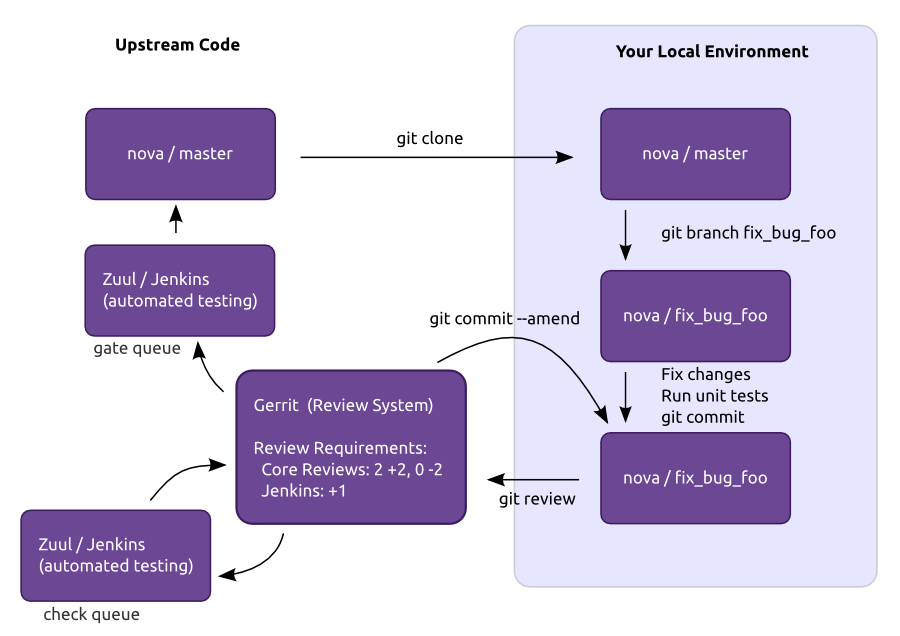
\includegraphics[width=.65\textwidth]{code_review.png}
  \end{center}
\end{frame}

\begin{frame}
  \frametitle{1つのパッチを投げると何が起こるのか?}
  \begin{center}
    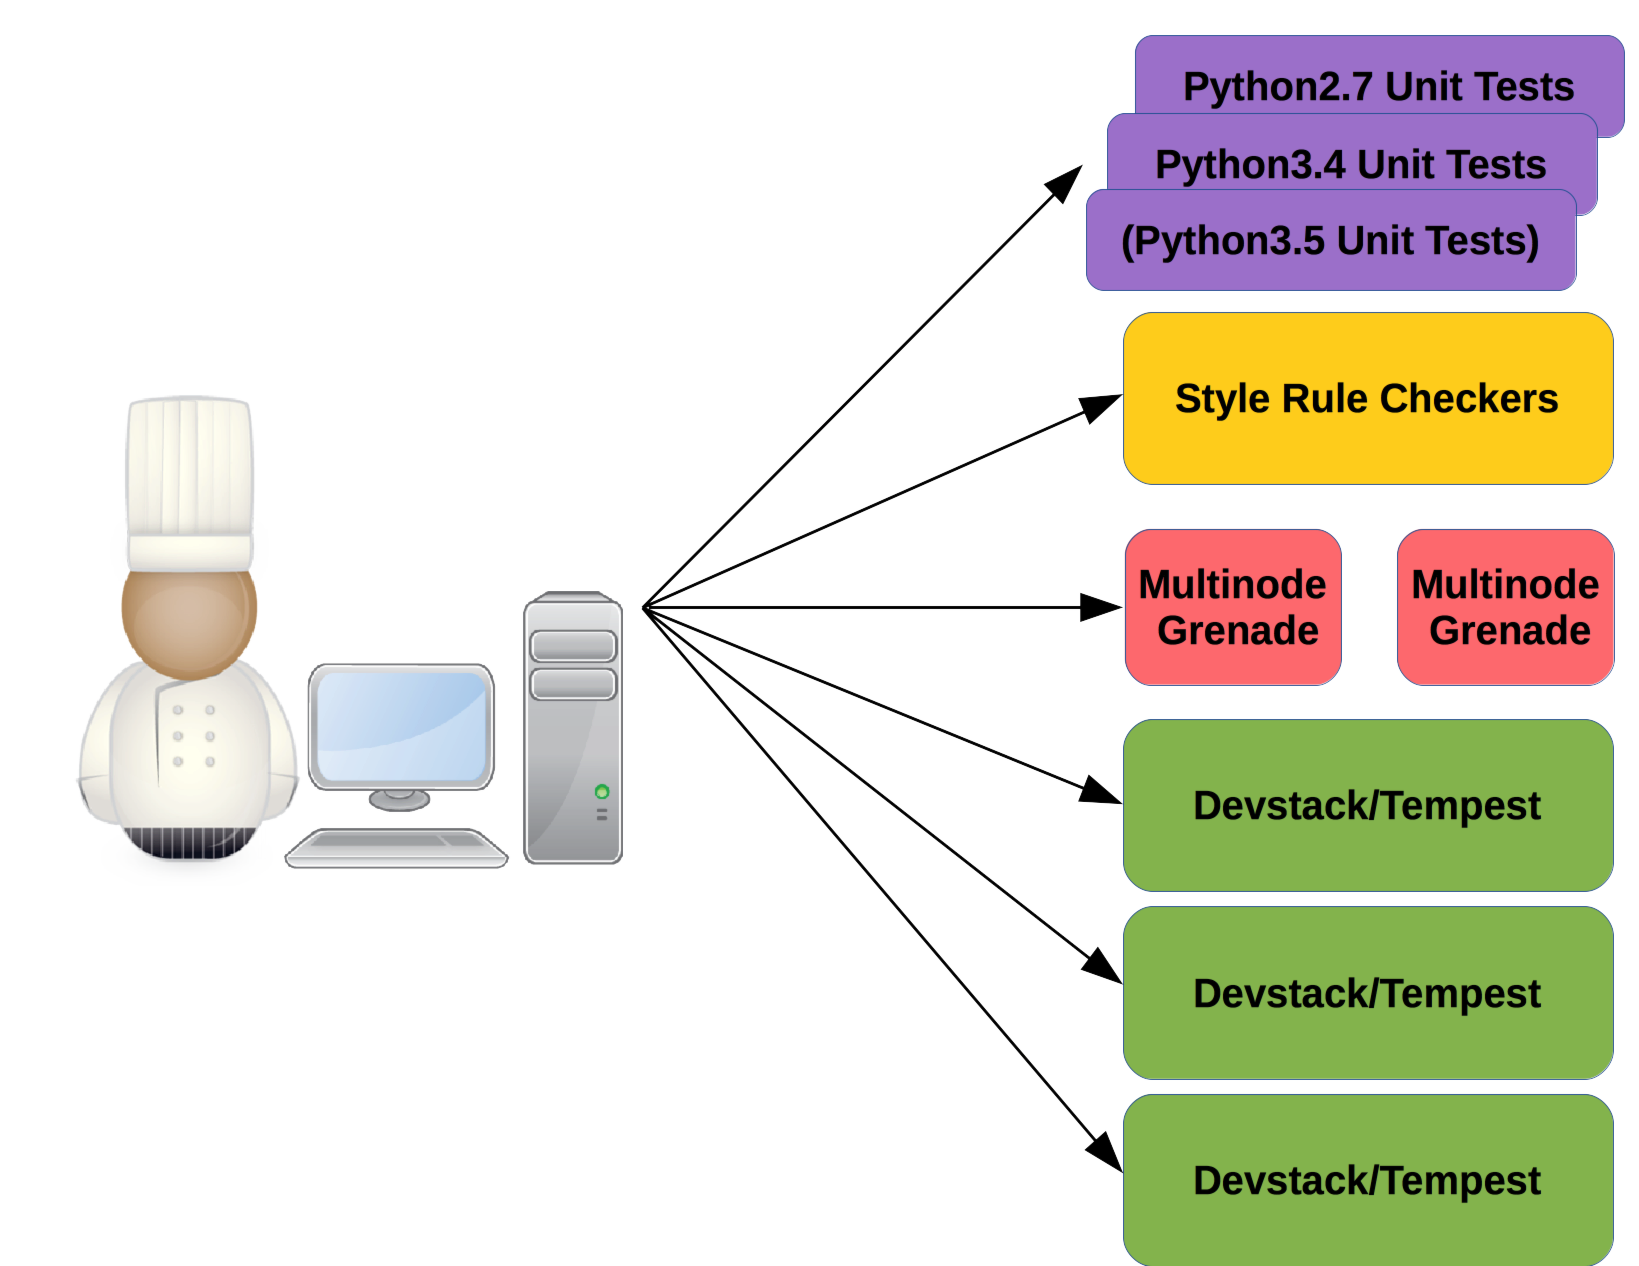
\includegraphics[width=.7\textwidth]{jobs.png}
  \end{center}
\end{frame}

\begin{frame}
  \begin{center}
      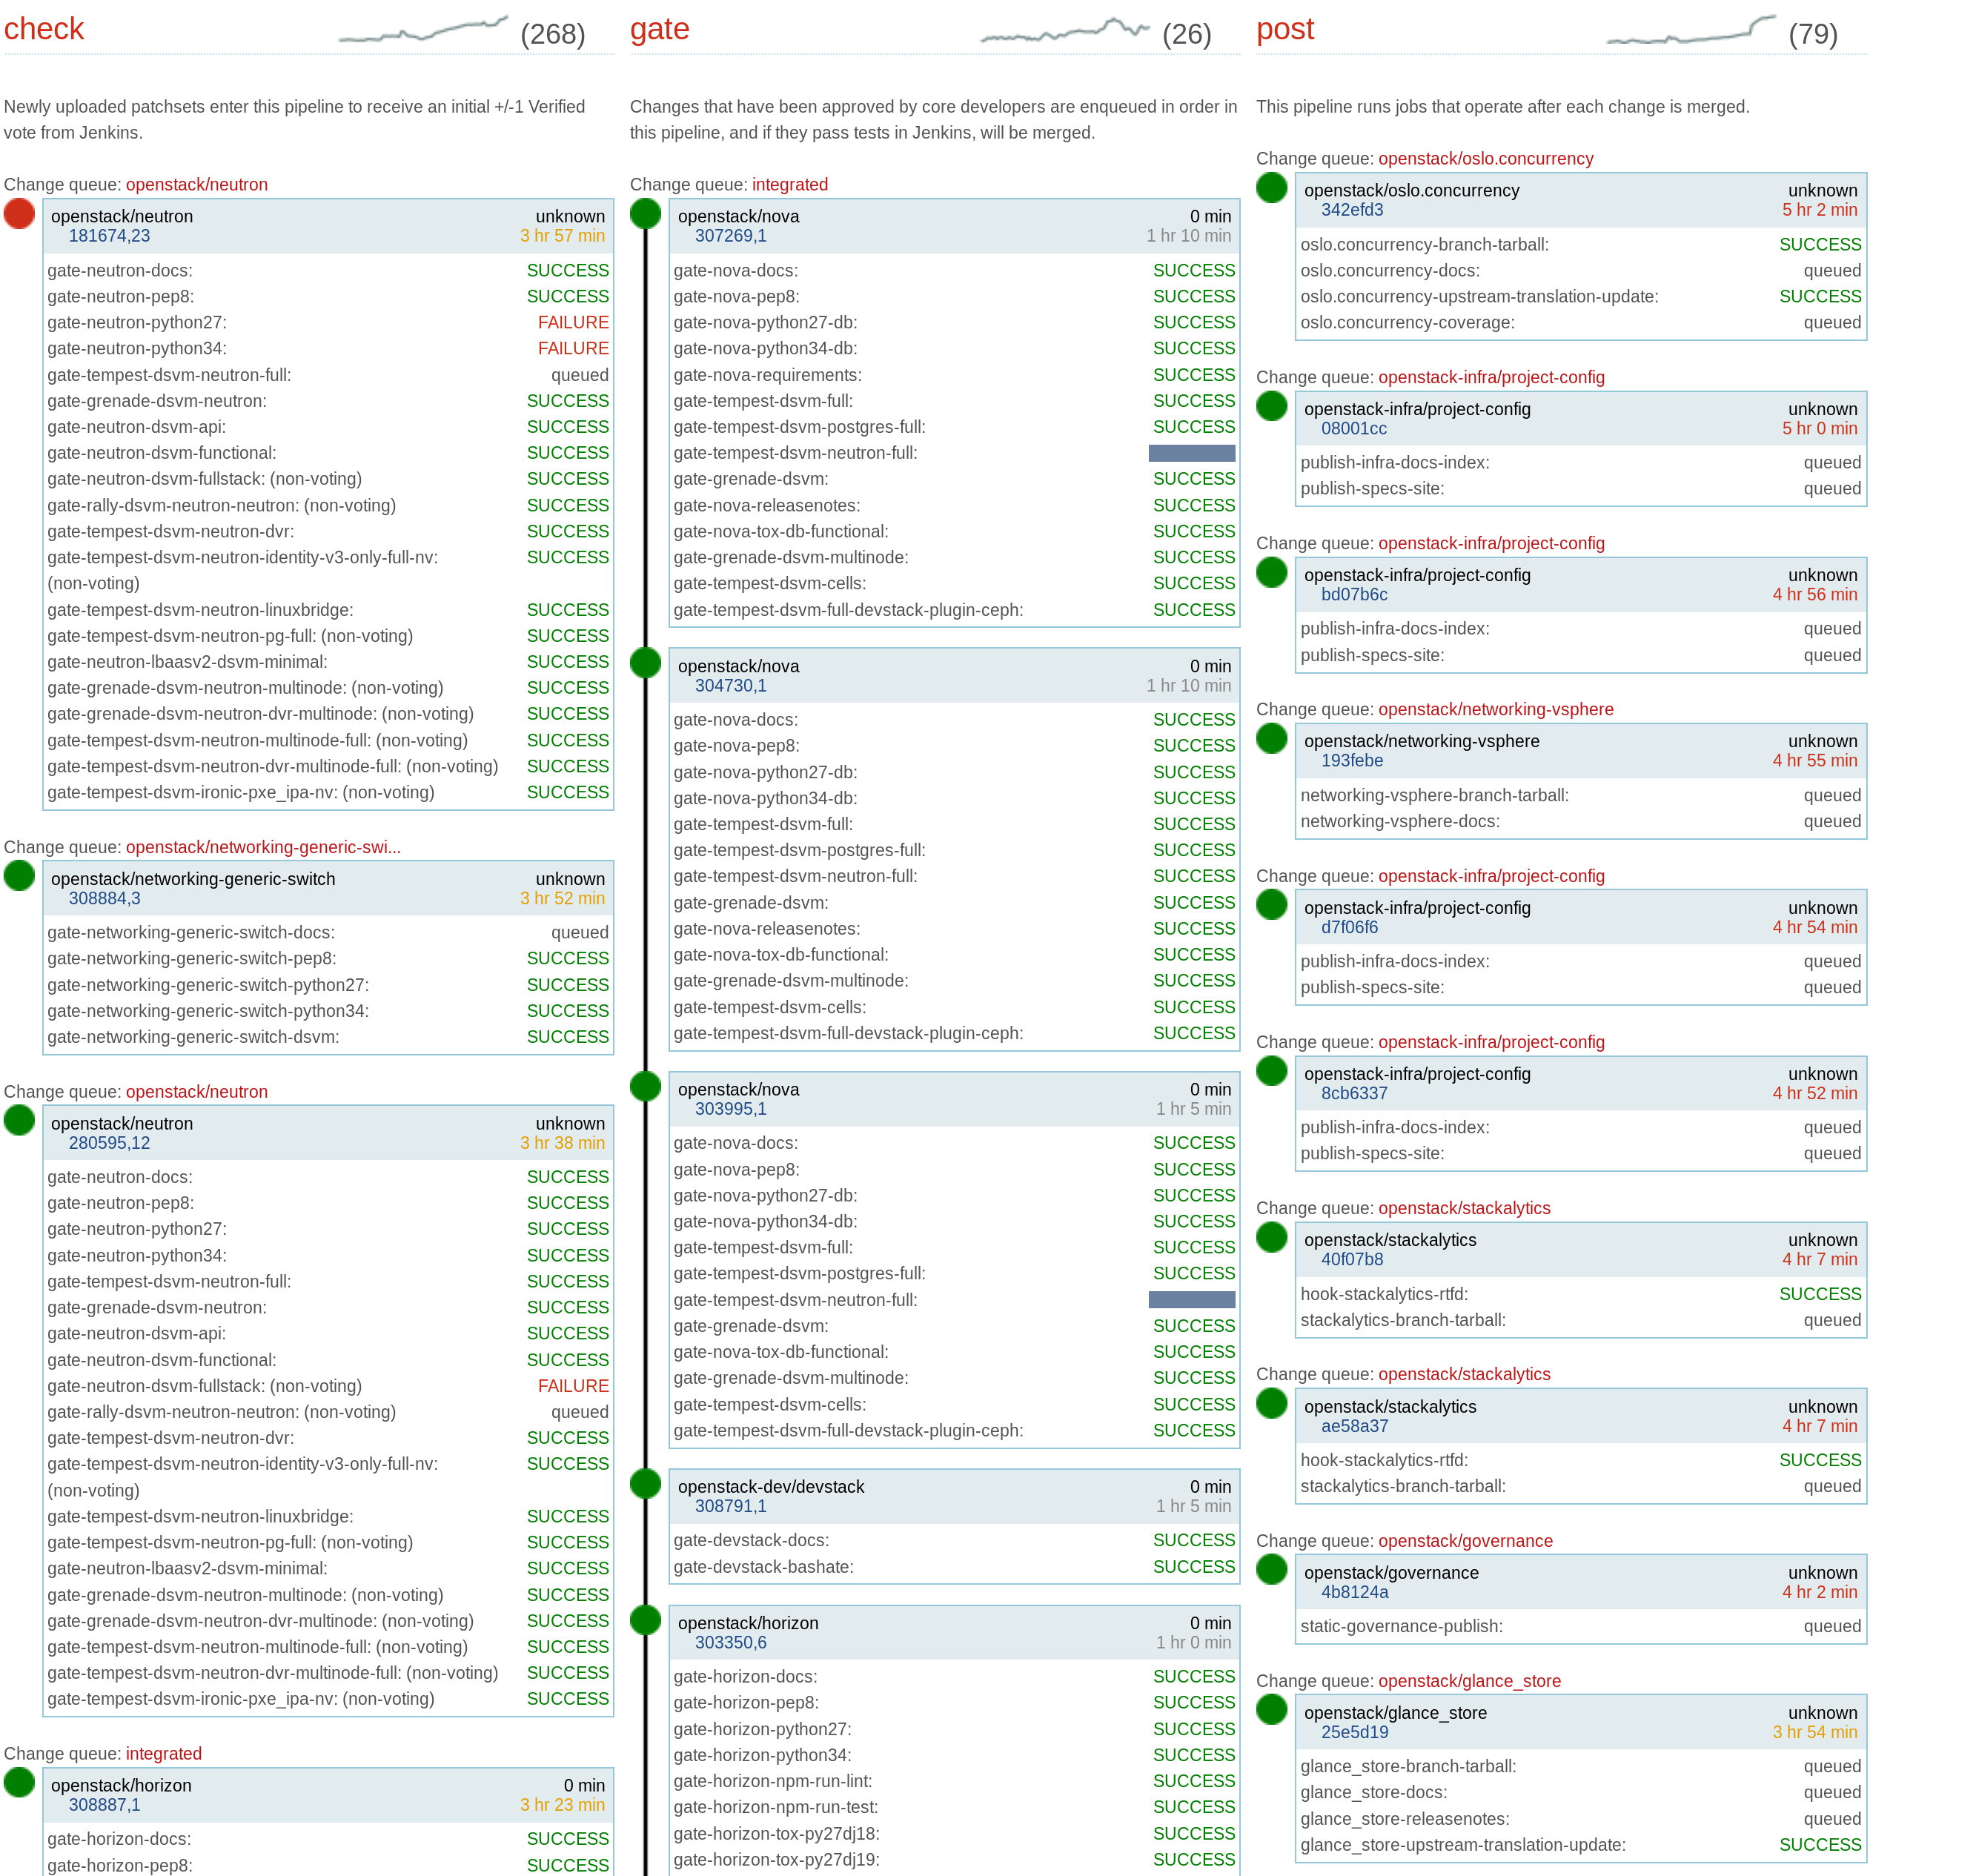
\includegraphics[width=.8\textwidth]{ZuulStatus.png}
  \end{center}
\end{frame}

\begin{frame}
\frametitle{Gateの規模感}
  \begin{columns}[T]
    \begin{column}{.50\textwidth}
      \textbf{1つのパッチで行われること:}
      \begin{itemize}
        \item 5--25 Devstacks
        \item \textasciitilde10,000 integration tests (約1.5k/devstack)
        \item \textasciitilde151 2ndレベルゲスト生成/devstack
        \item \textasciitilde1 GBログファイル (非圧縮時)/実行毎
      \end{itemize}
      \textbf{合計すると:}
      \begin{itemize}
        \item \textasciitilde12,500 ジョブ (check or gate)実行/日
        \item \textasciitilde0.01\% 個別tempestテスト毎 失敗率
        \item \textasciitilde.77\% tempest 実行全体 失敗率
      \end{itemize}
    \end{column}
    \begin{column}{.48\textwidth}
        \centering
        \textbf{Tempestテスト実行数/日 (GateQ):}
        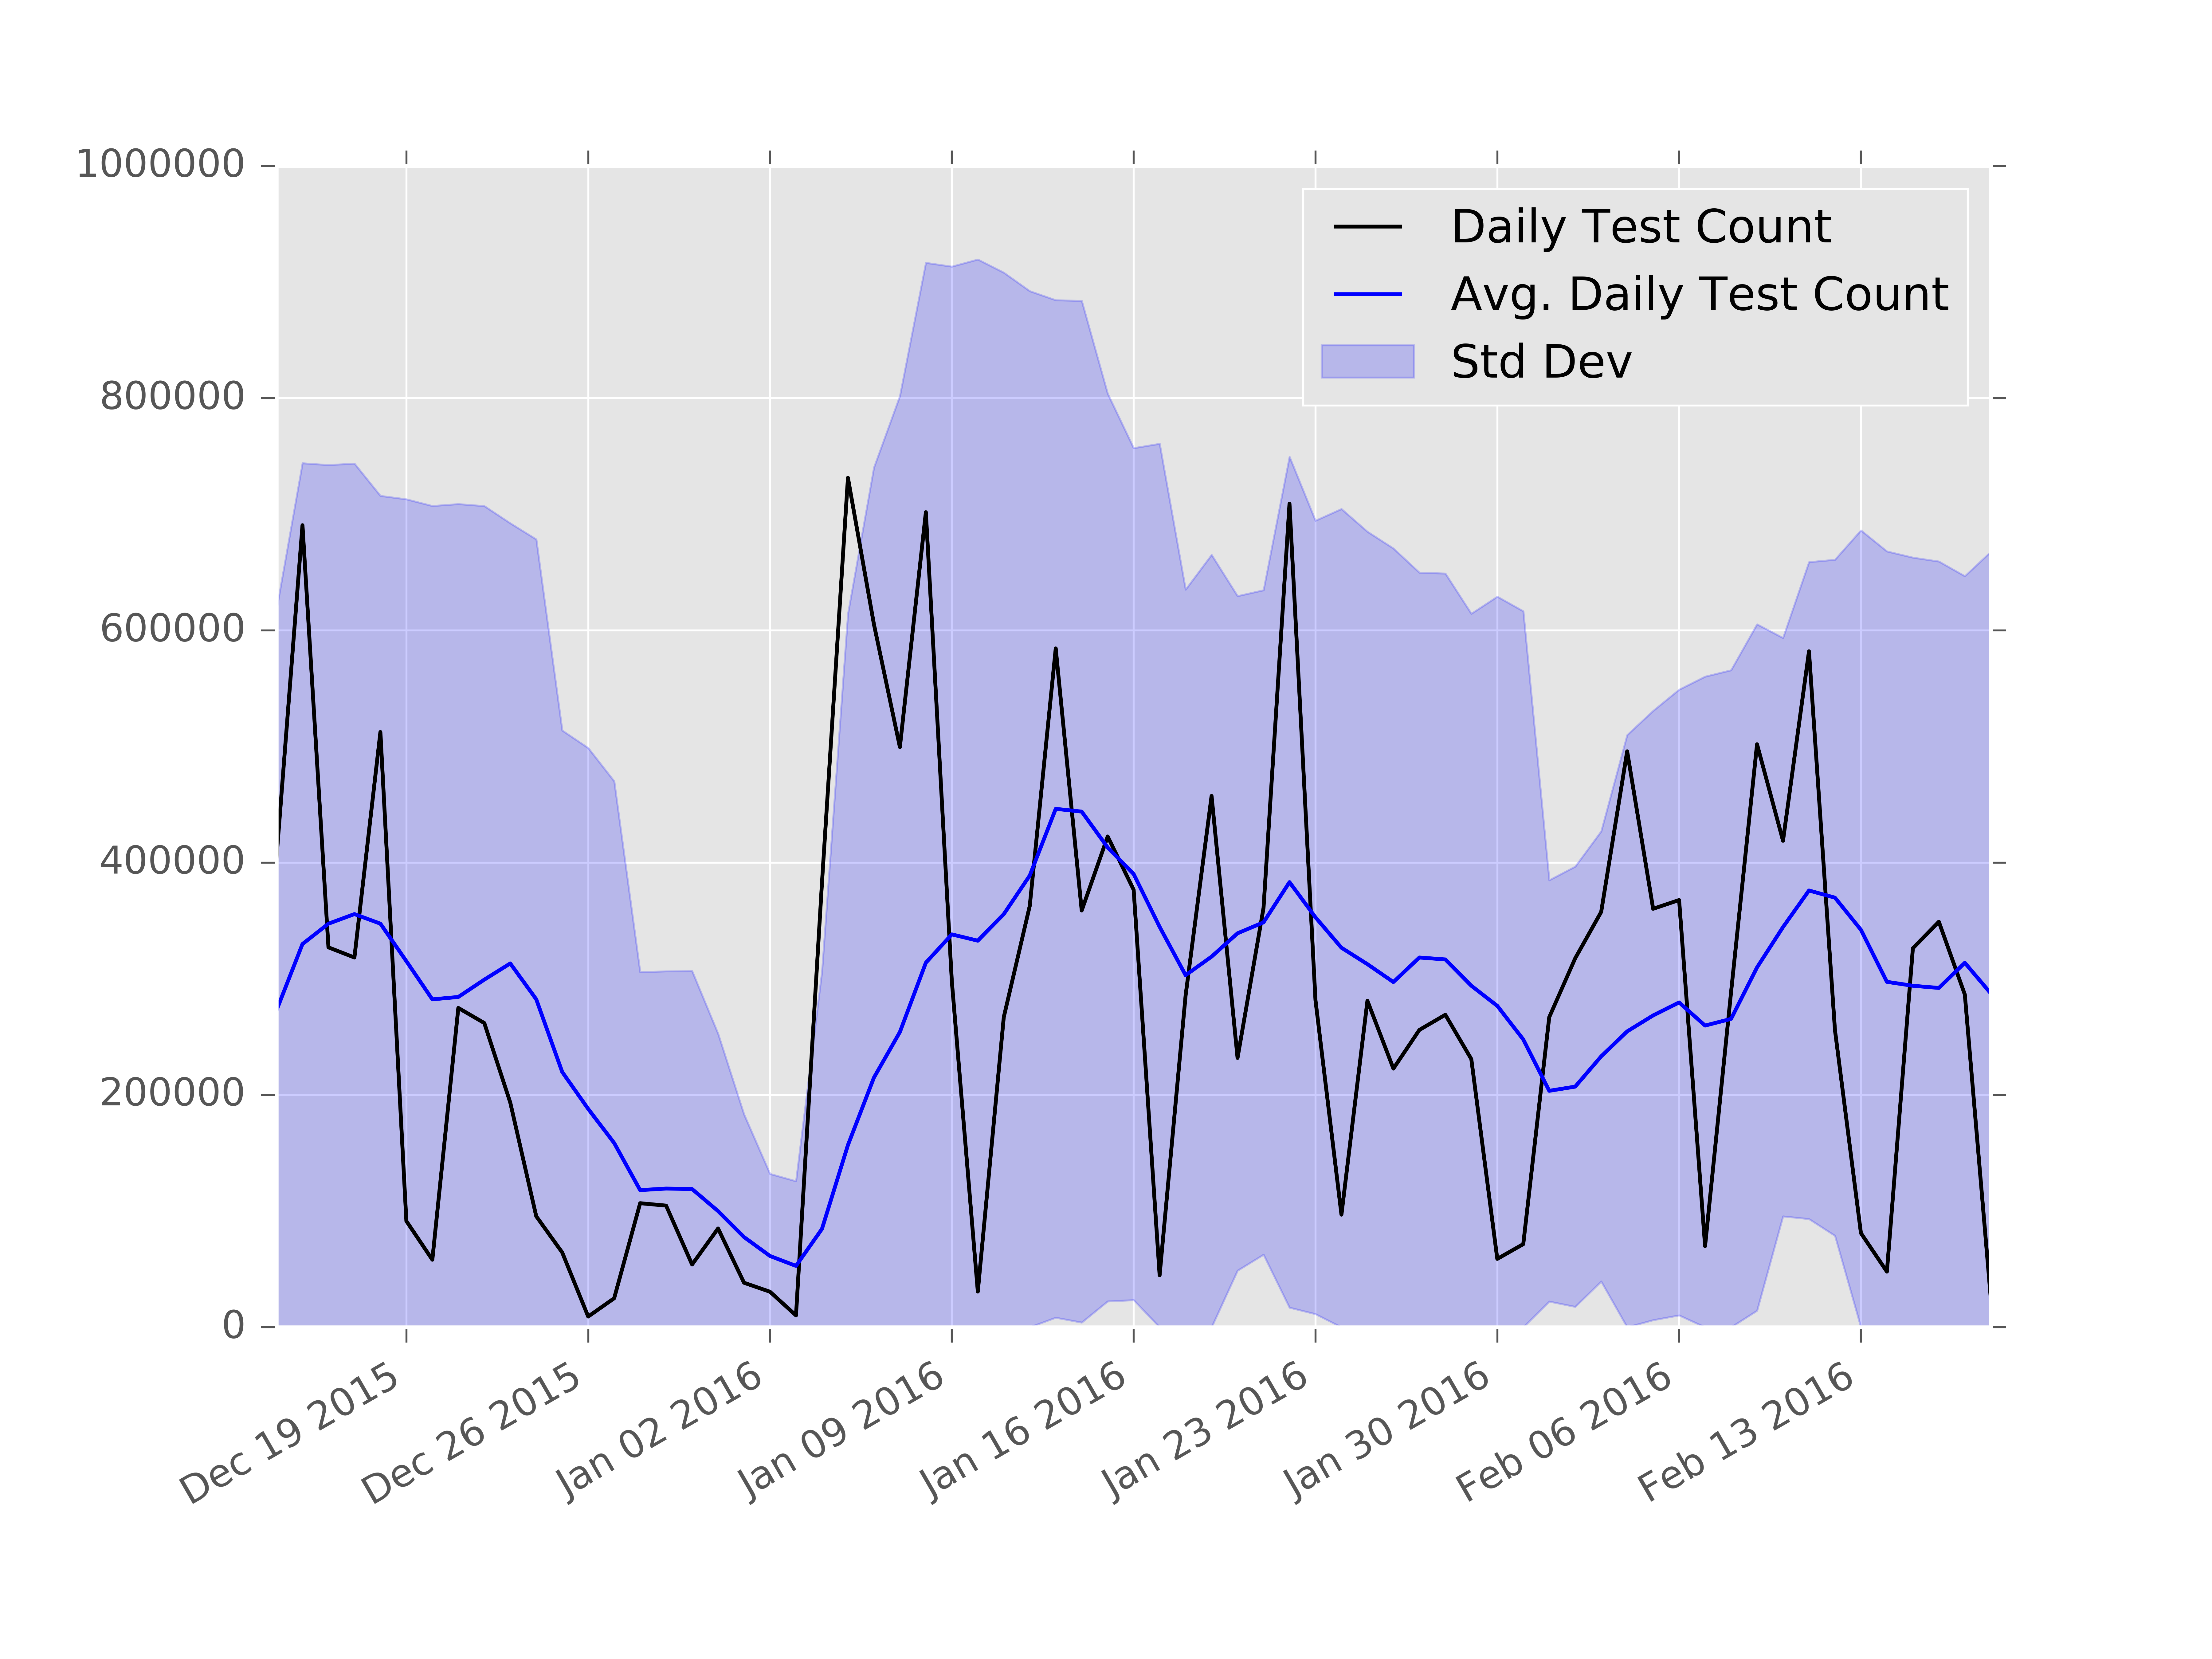
\includegraphics[width=1.22\textwidth]{tempest-gate-count.png}
    \end{column}
  \end{columns}
\end{frame}

\subsection{Complications with the Size}
\begin{frame}
  \frametitle{Log Server}
  \begin{itemize}
    \item Log Server: \href{http://logs.openstack.org/}{logs.openstack.org}
    \item 全ジョブの生成物を\textasciitilde4ヶ月保持
%http://cacti.openstack.org/cacti/graph.php?action=view&local_graph_id=717&rra_id=all
    \item \textasciitilde8 TBの圧縮データ
  \end{itemize}
  \begin{center}
    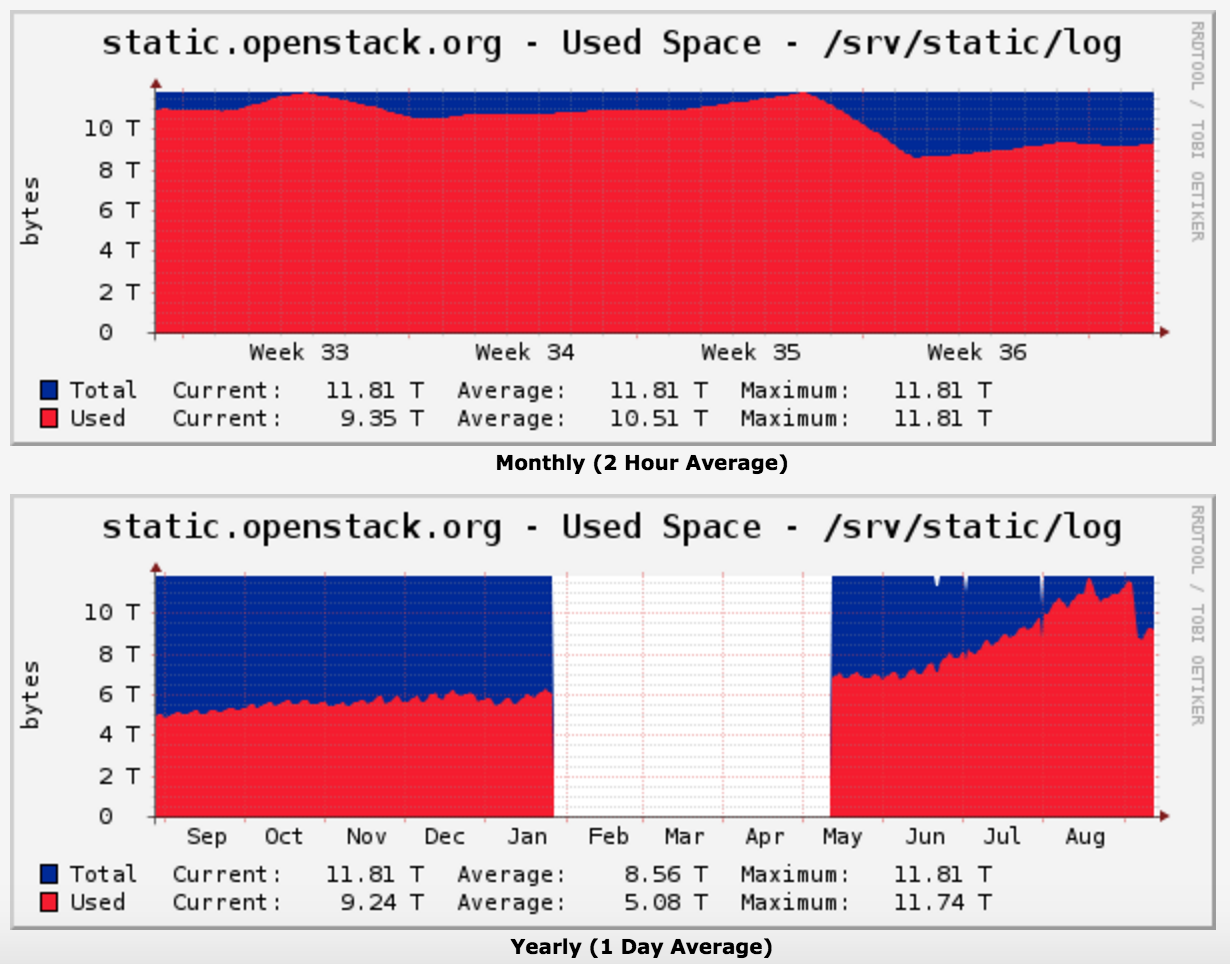
\includegraphics[width=.55\textwidth]{cacti-static-openstack-org-log-graph.png}
  \end{center}
\end{frame}

\begin{frame}
  \frametitle{困ったこと}
  \begin{itemize}
    \item 大量のログの中から目的のものを見つける必要あり
    \item 大量のテスト実行結果を俯瞰的に確認したい (パフォーマンス劣化・向上の検出等)
    \item どのくらいの頻度で成功/失敗しているかを知ることが困難
  \end{itemize}
\end{frame}

\section{Solutions}
\begin{frame}
  \frametitle{一般的なアプローチ}
    \begin{itemize}
        \item より大きな視点で、大局的に物事を見る
        \item 統計情報やデータマイニングをして、未知の傾向を見つけ出す
        \item テスト実行結果をオープンにして、誰もが見られるようにする
        \item 全ての情報にアクセスできるAPIを確保する
    \end{itemize}
\end{frame}

\begin{frame}
  \frametitle{Graphite}
  \begin{itemize}
    \item \href{http://graphite.openstack.org/}{graphite.openstack.org}
    \item OpenStack Infra チームが提供
    \item Include job results
    \item Jobレベルのデータに限定
    \item 個別のJobへのリンクはできない
  \end{itemize}
  \begin{center}
    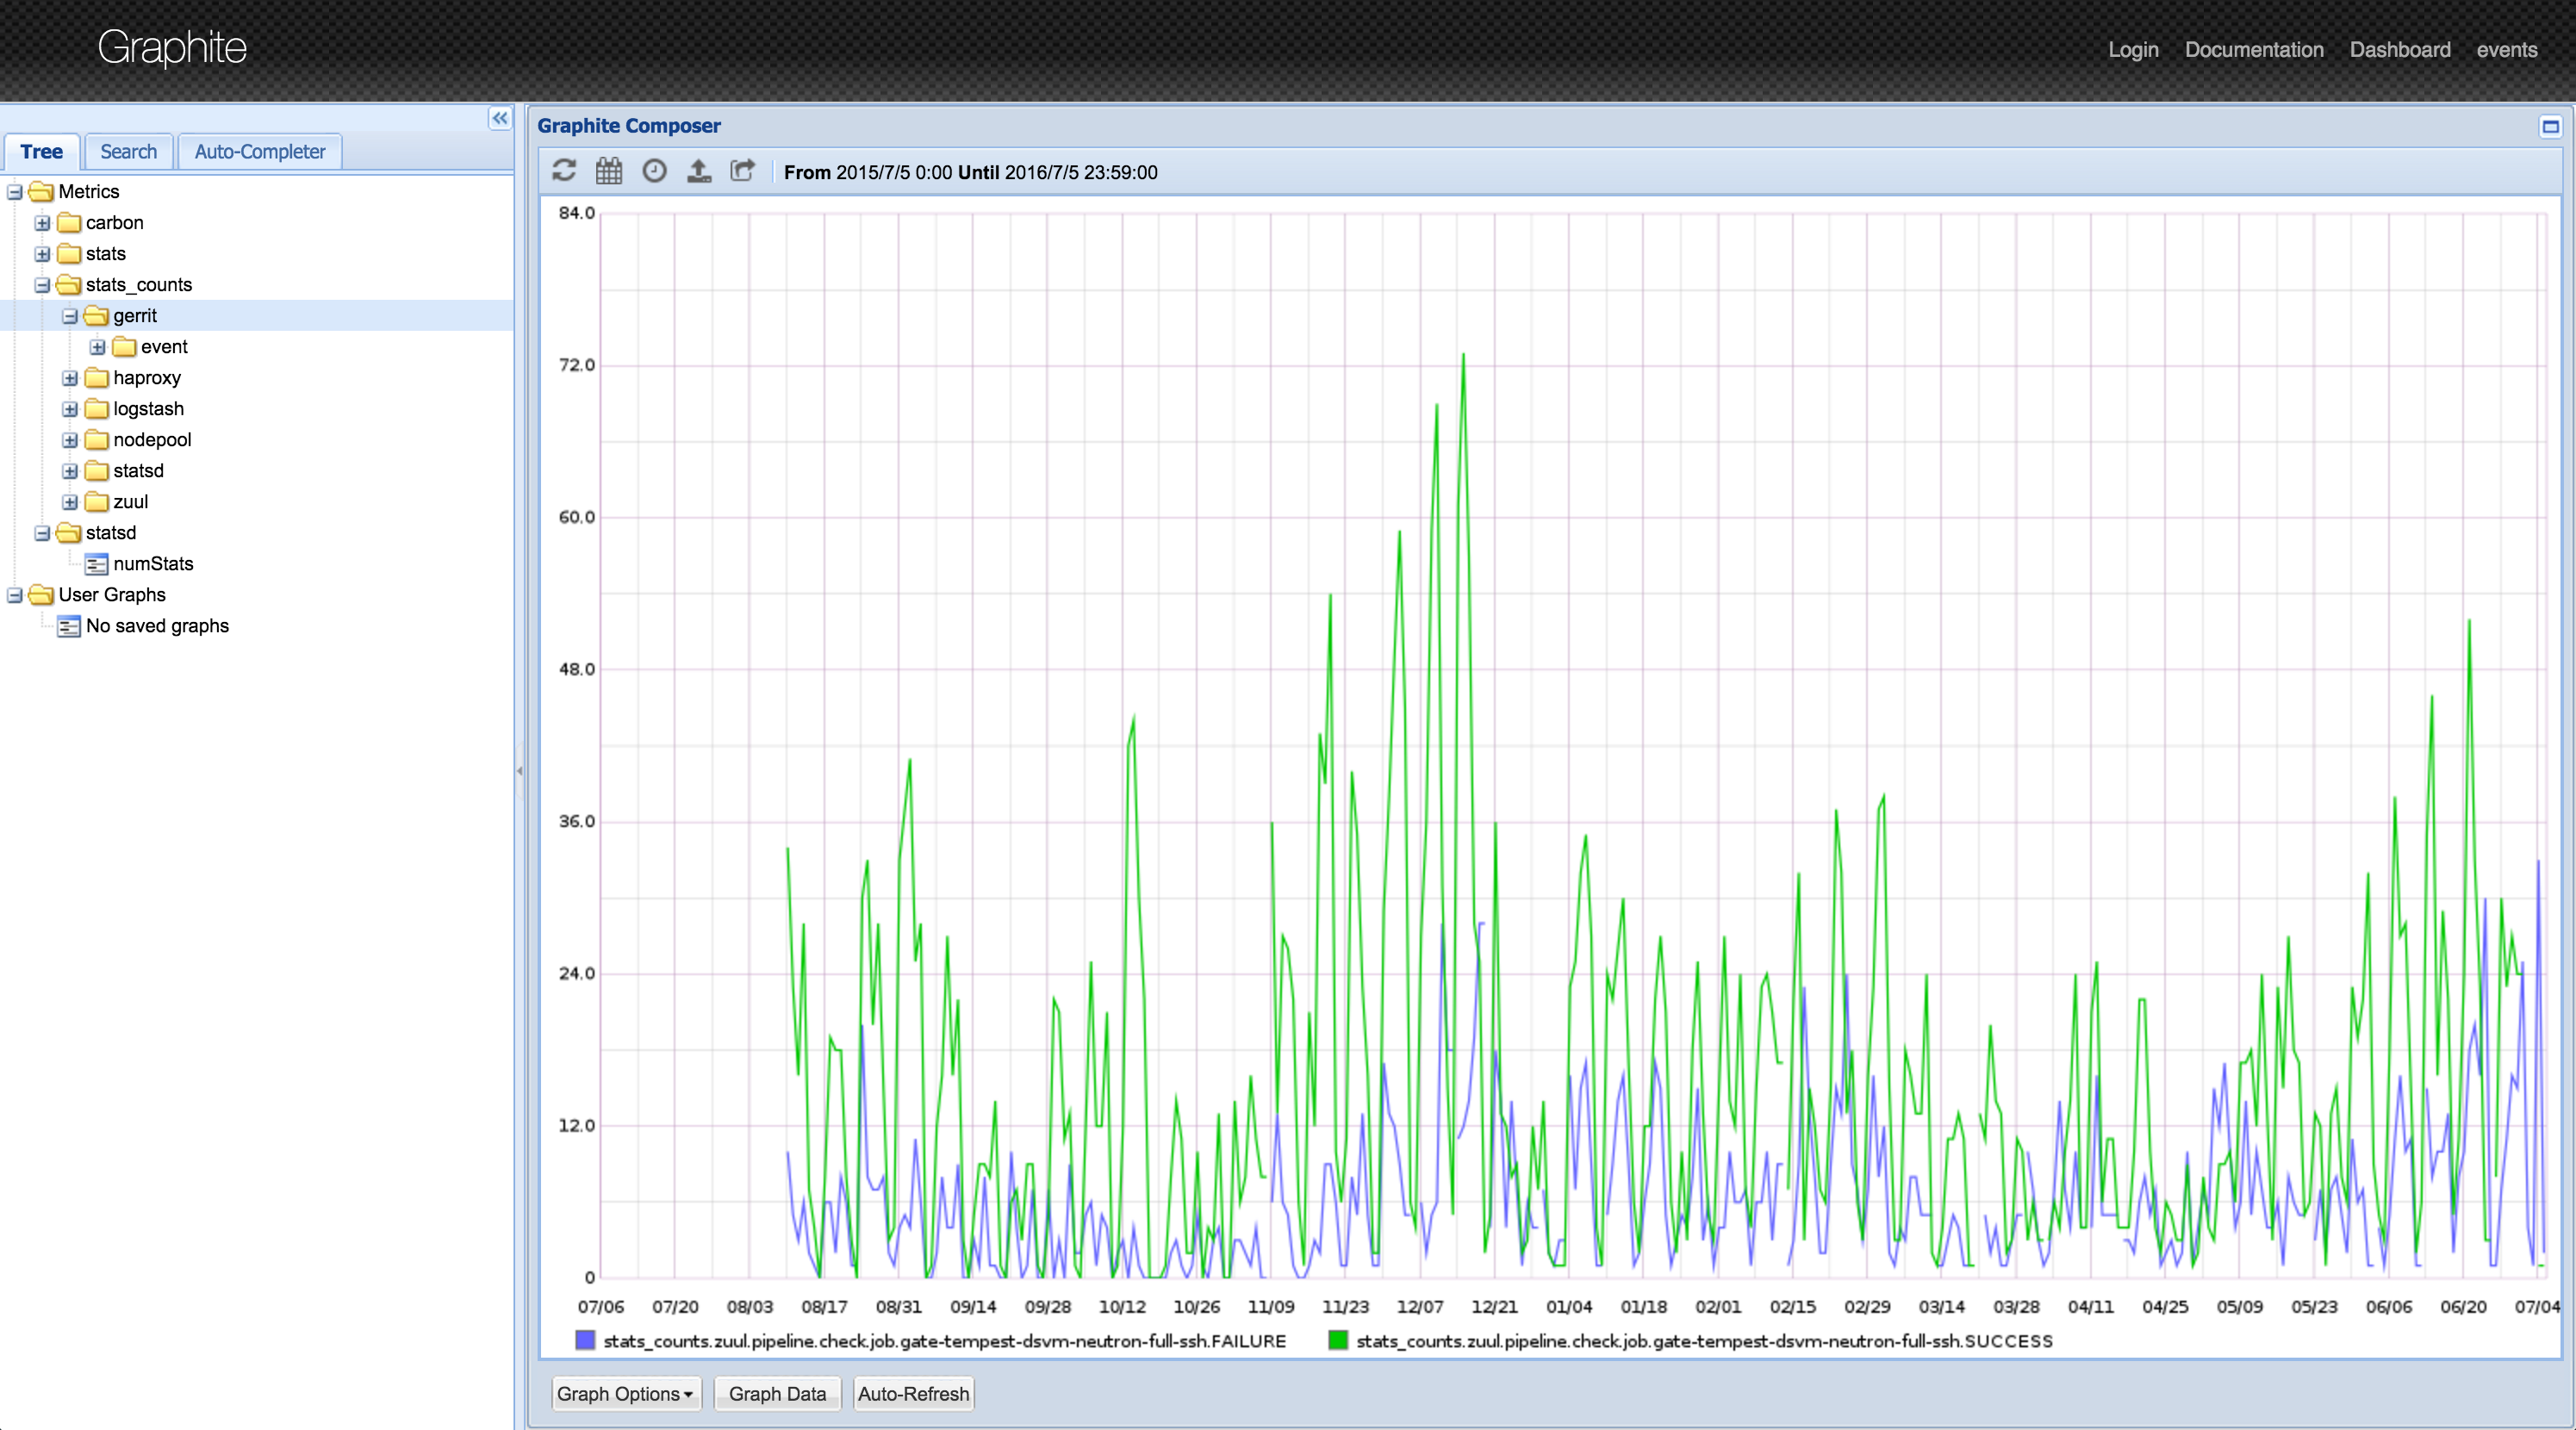
\includegraphics[width=.65\textwidth]{graphite-sample.png}
  \end{center}
\end{frame}

\begin{frame}
  \frametitle{Grafana}
  \begin{itemize}
    \item \href{http://grafana.openstack.org/}{grafana.openstack.org}
    \item Graphiteに対するDashboard機能を提供 (簡単に視覚化できる)
    \item 既にいくつかのダッシュボードが提供されている
    \item 数プロジェクト(Neutron等)がJob失敗率視覚化に利用中
  \end{itemize}
  \begin{center}
    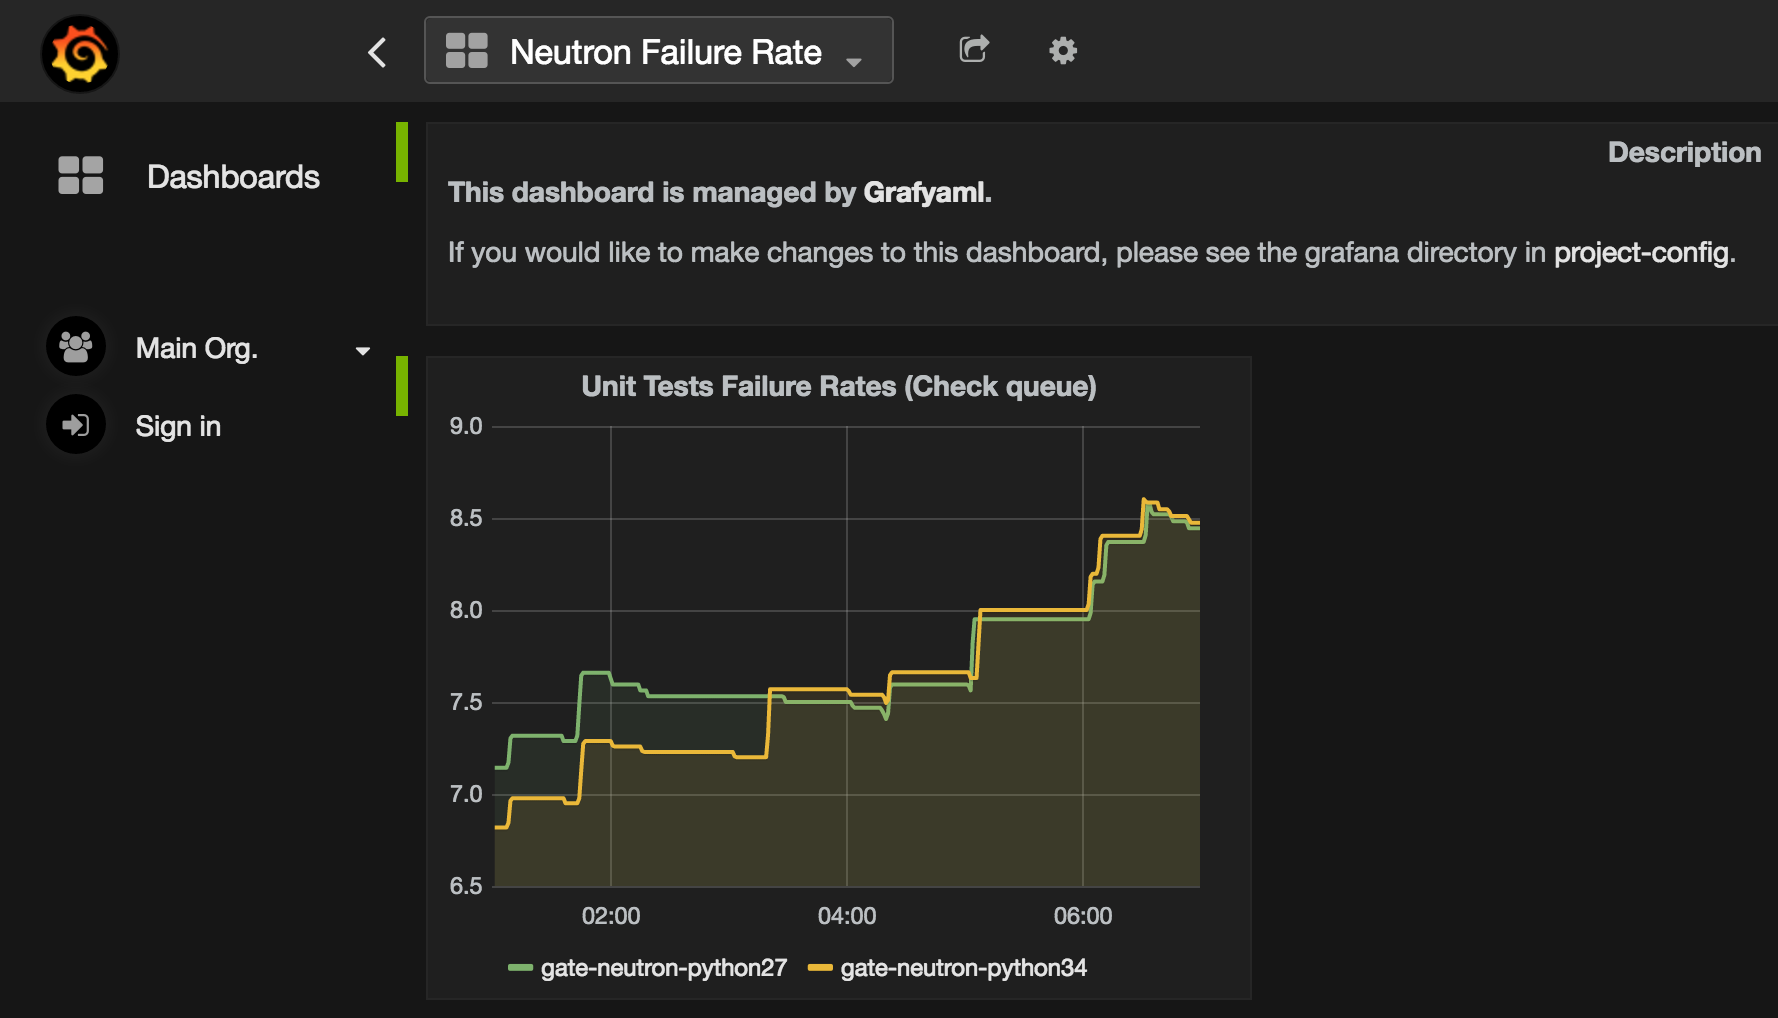
\includegraphics[width=.7\textwidth]{grafana-sample.png}
  \end{center}
\end{frame}

\section{Solutions to Size issues}
\begin{frame}
  \frametitle{ELK}
  \begin{itemize}
    \item Elasticsearch, Logstash, Kibana
    \item \href{http://logstash.openstack.org}{logstash.openstack.org}
    \item 大量のログファイルを検索する機能を提供
    \item 10日間のログデータに制限
  \end{itemize}
  \begin{center}
    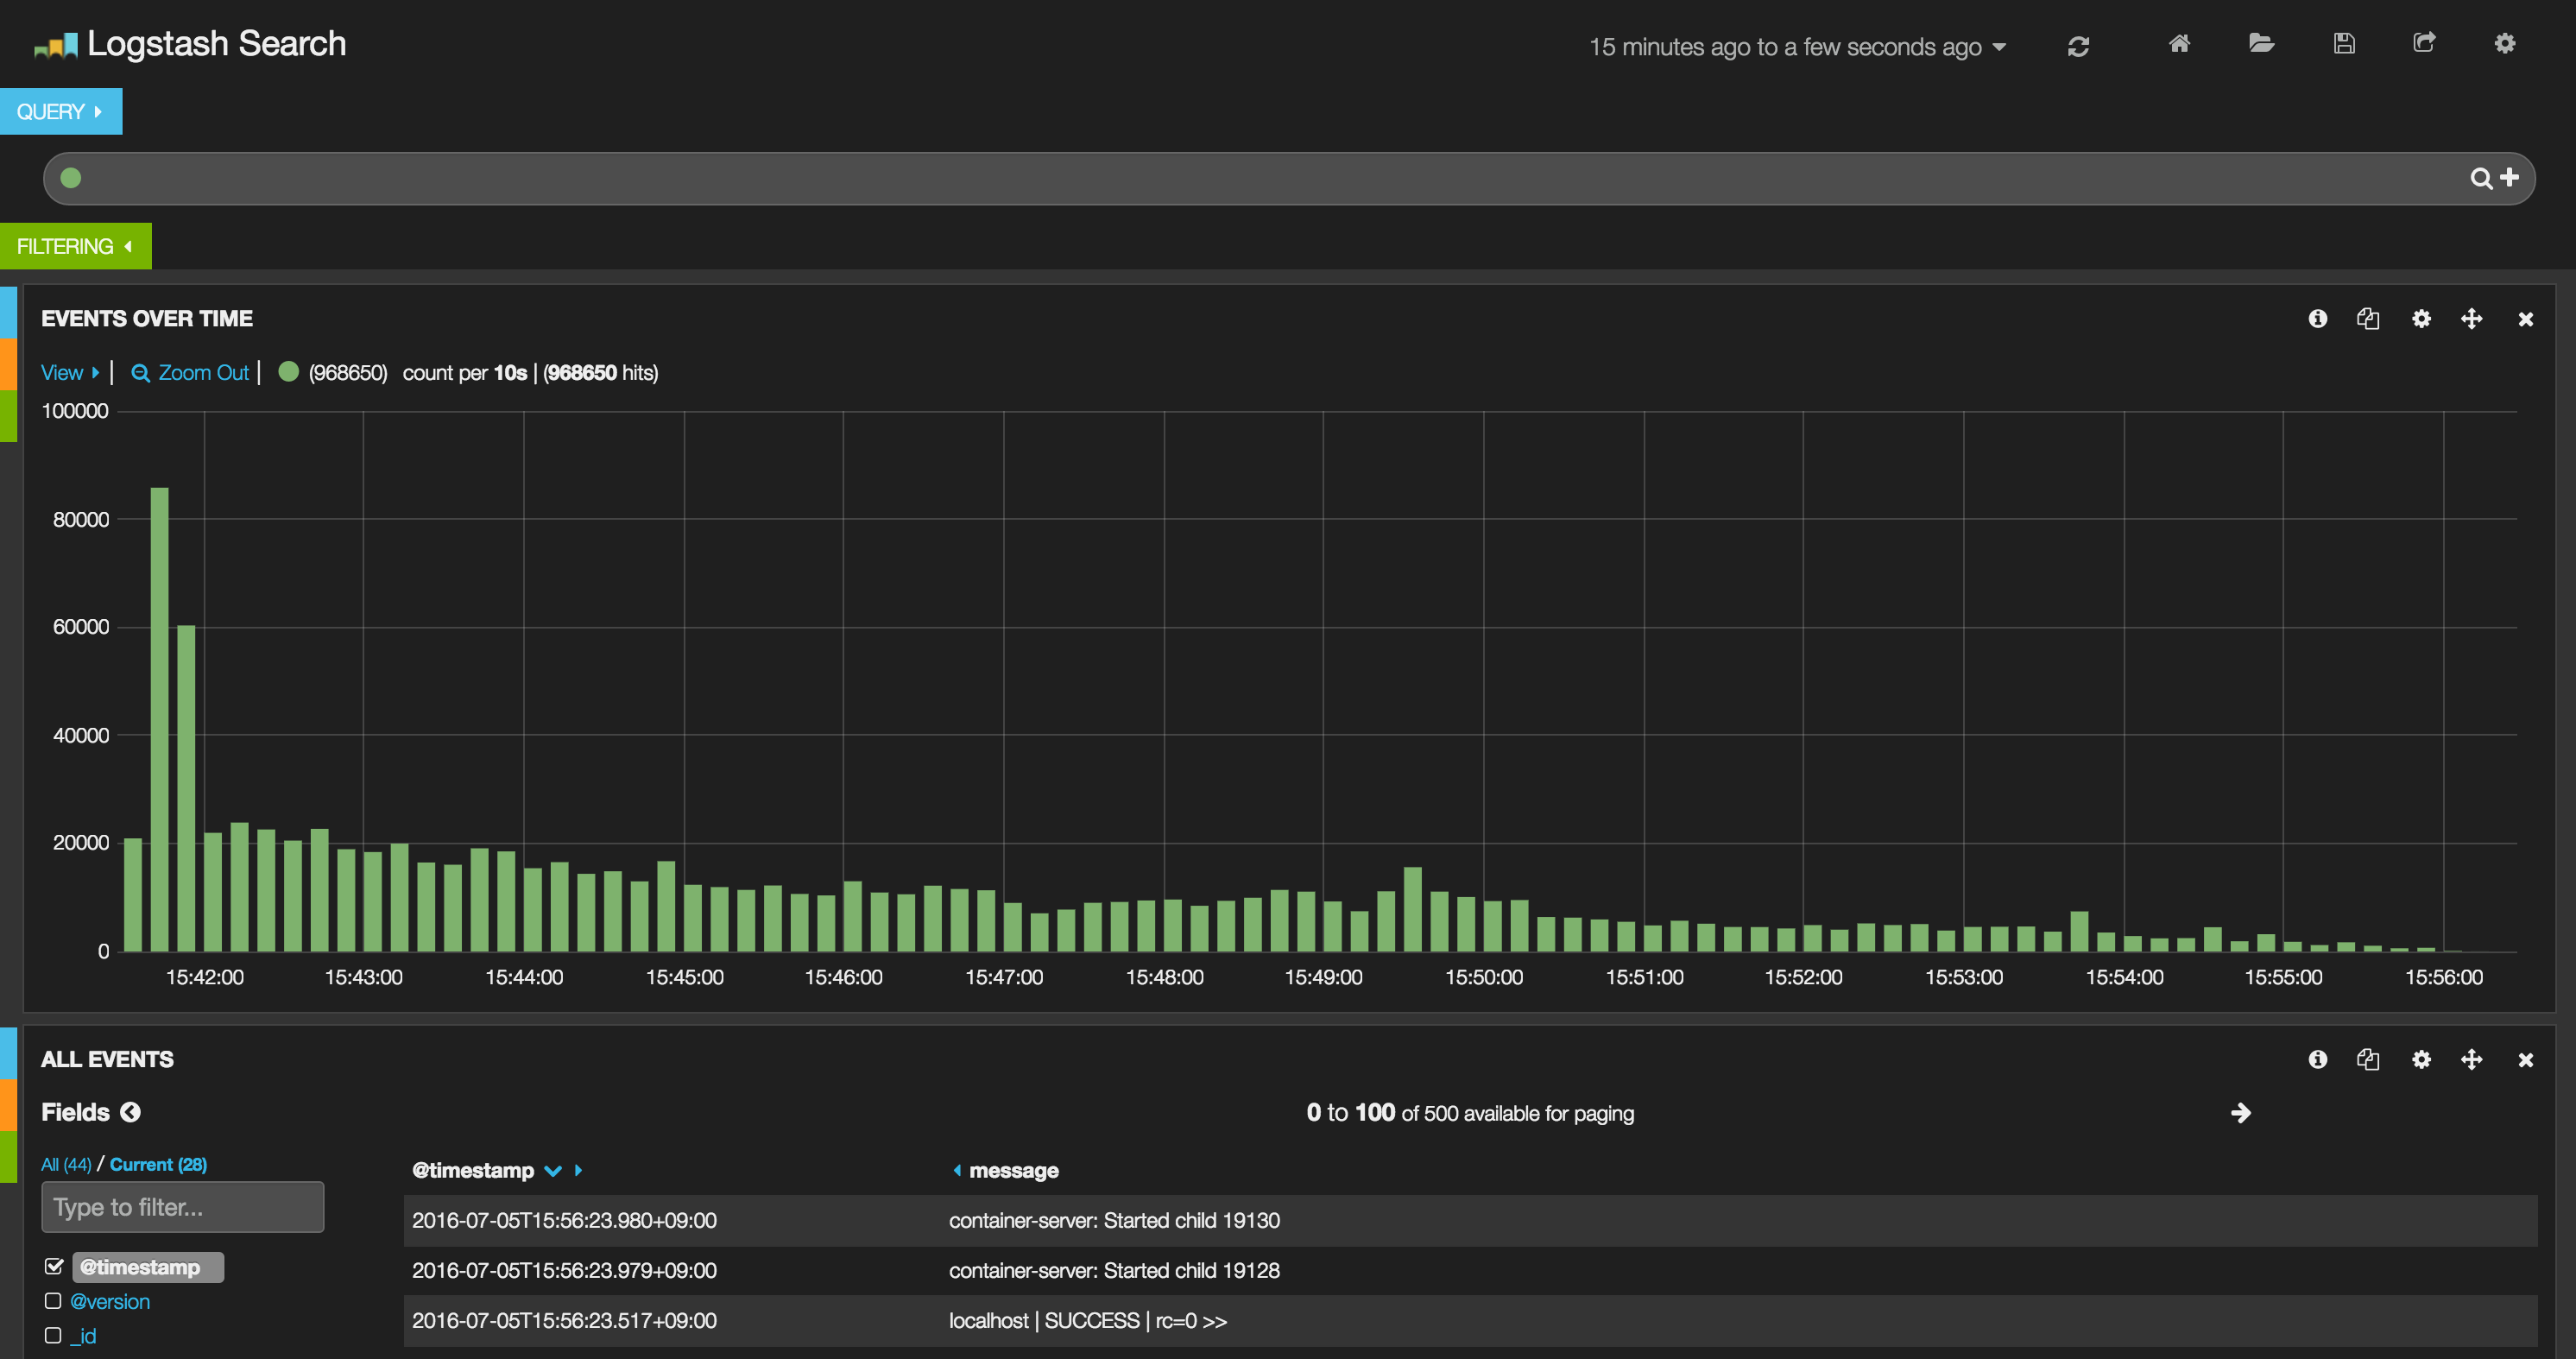
\includegraphics[width=.75\textwidth]{kibana-sample.png}
  \end{center}
\end{frame}

\begin{frame}
  \frametitle{openstack-health}
  \begin{itemize}
    \item \href{http://status.openstack.org/openstack-health/}{status.openstack.org/openstack-health}
    \item ゲートの実行結果データをアクセスできるダッシュボードとして開発開始
    \item subunit2sqlとelastic recheckのデータと連携
  \end{itemize}
  \begin{center}
    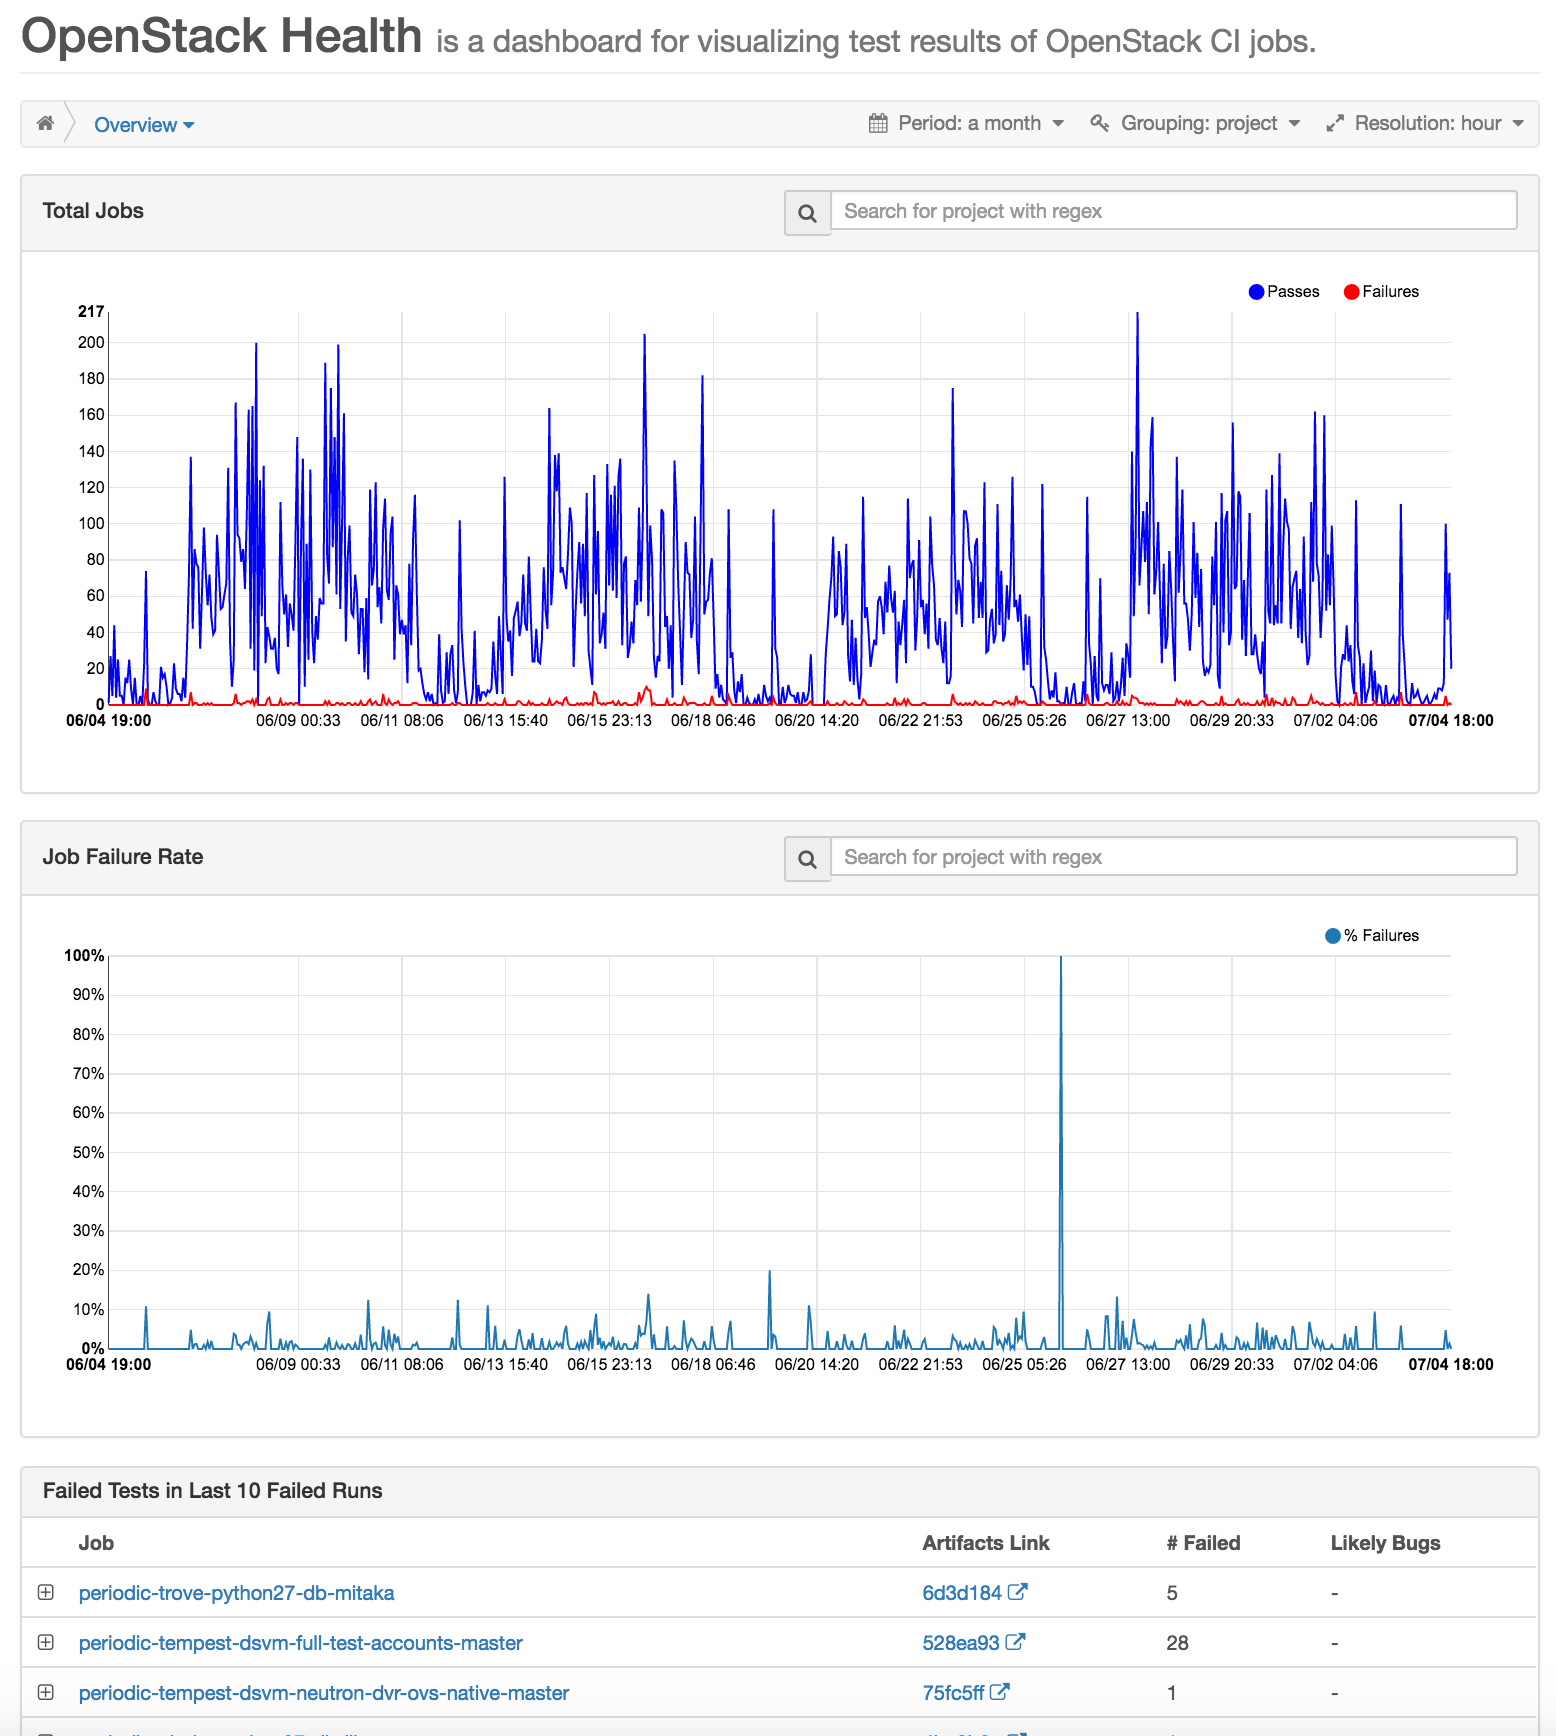
\includegraphics[height=0.6\textheight]{openstack-health-1.png}
    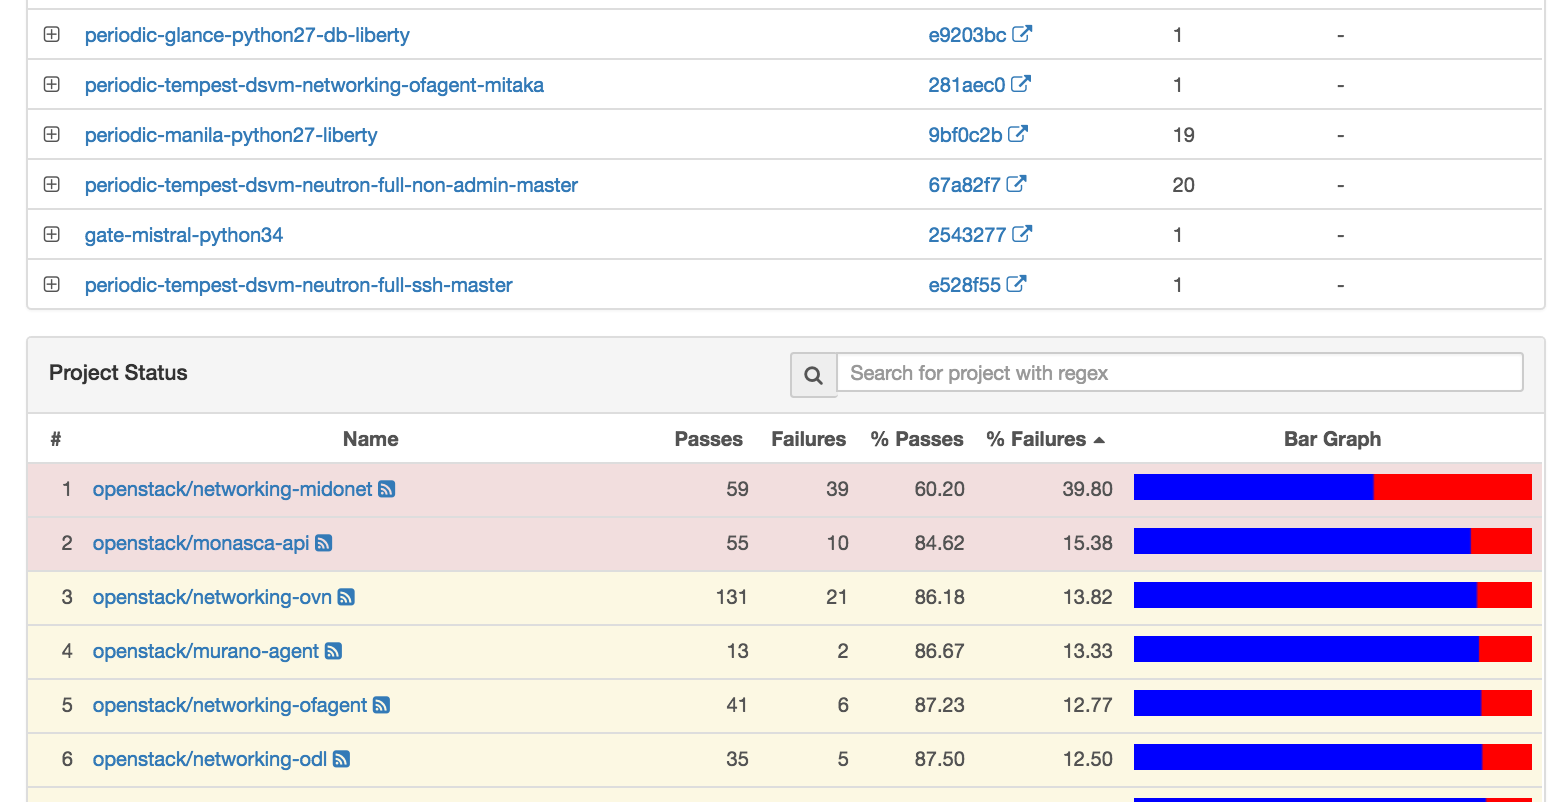
\includegraphics[height=0.6\textheight]{openstack-health-2.png}
  \end{center}
\end{frame}

\begin{frame}
  \frametitle{OpenStack-Health Architecture}
  \begin{center}
    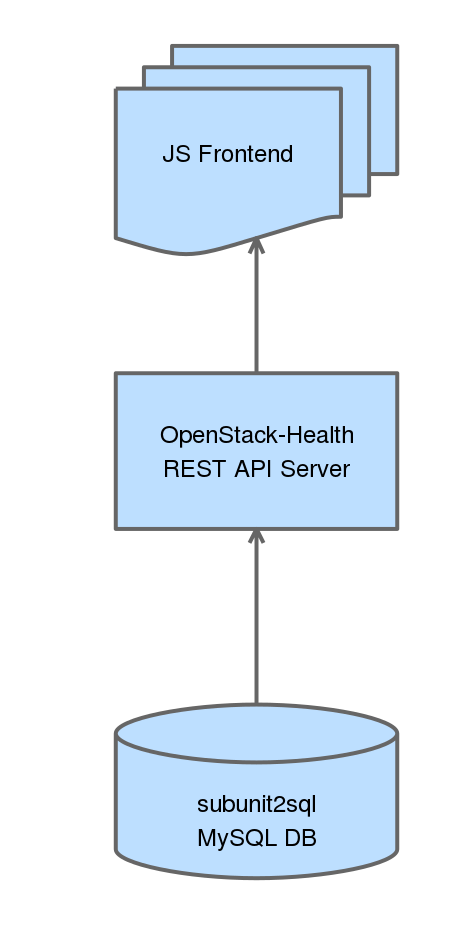
\includegraphics[height=1.2\textheight]{openstack-health-arch.png}
  \end{center}
\end{frame}

\begin{frame}
  \frametitle{subunit2sql}
  \begin{itemize}
    \item テスト結果データをSQLデータベースに保持する機能を提供
    \item 対応DB: MySQL, PostgreSQL, SQLite
    \item DBに保持したデータに対するPython APIを提供
    \item 6ヶ月間の実行結果を保持(ゲート環境)
  \end{itemize}
\end{frame}

\begin{frame}
  \frametitle{subunit2sql in OpenStackインフラ}
  \begin{center}
    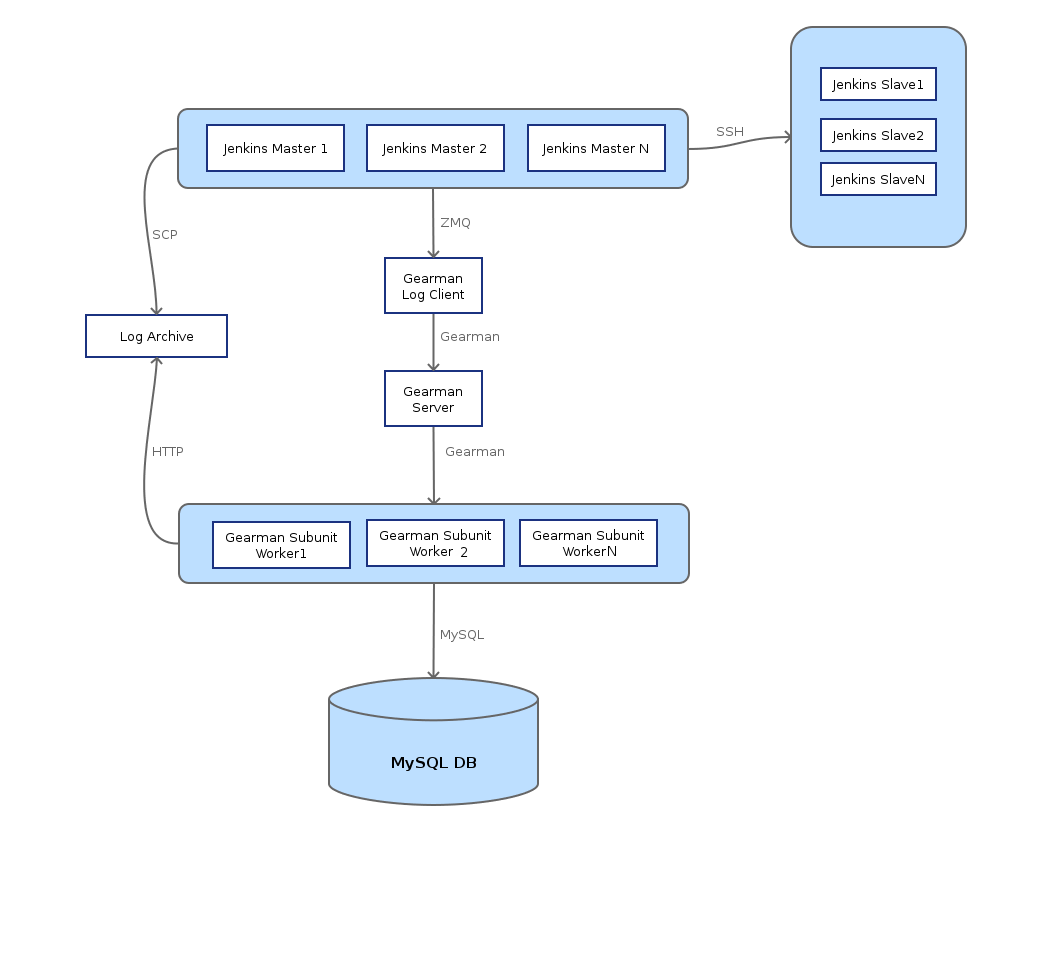
\includegraphics[height=1.1\textheight]{subunit2sql-collection.png}
  \end{center}
\end{frame}

\begin{frame}
  \frametitle{Elastic Recheck}
  \begin{itemize}
    \item 「このエラー前にも起きたよね?」を自動的に検出する
    \item \href{http://status.openstack.org/elastic-recheck/}{status.openstack.org/elastic-recheck}
    \item 以下の2つで構成:
      \begin{itemize}
        \item ボット: 変更・レポートを監視して、失敗を検知してGerrit/IRCへ通知
        \item ダッシュボード: 失敗をカテゴライズしたものを表示
      \end{itemize}
  \end{itemize}
  \begin{center}
    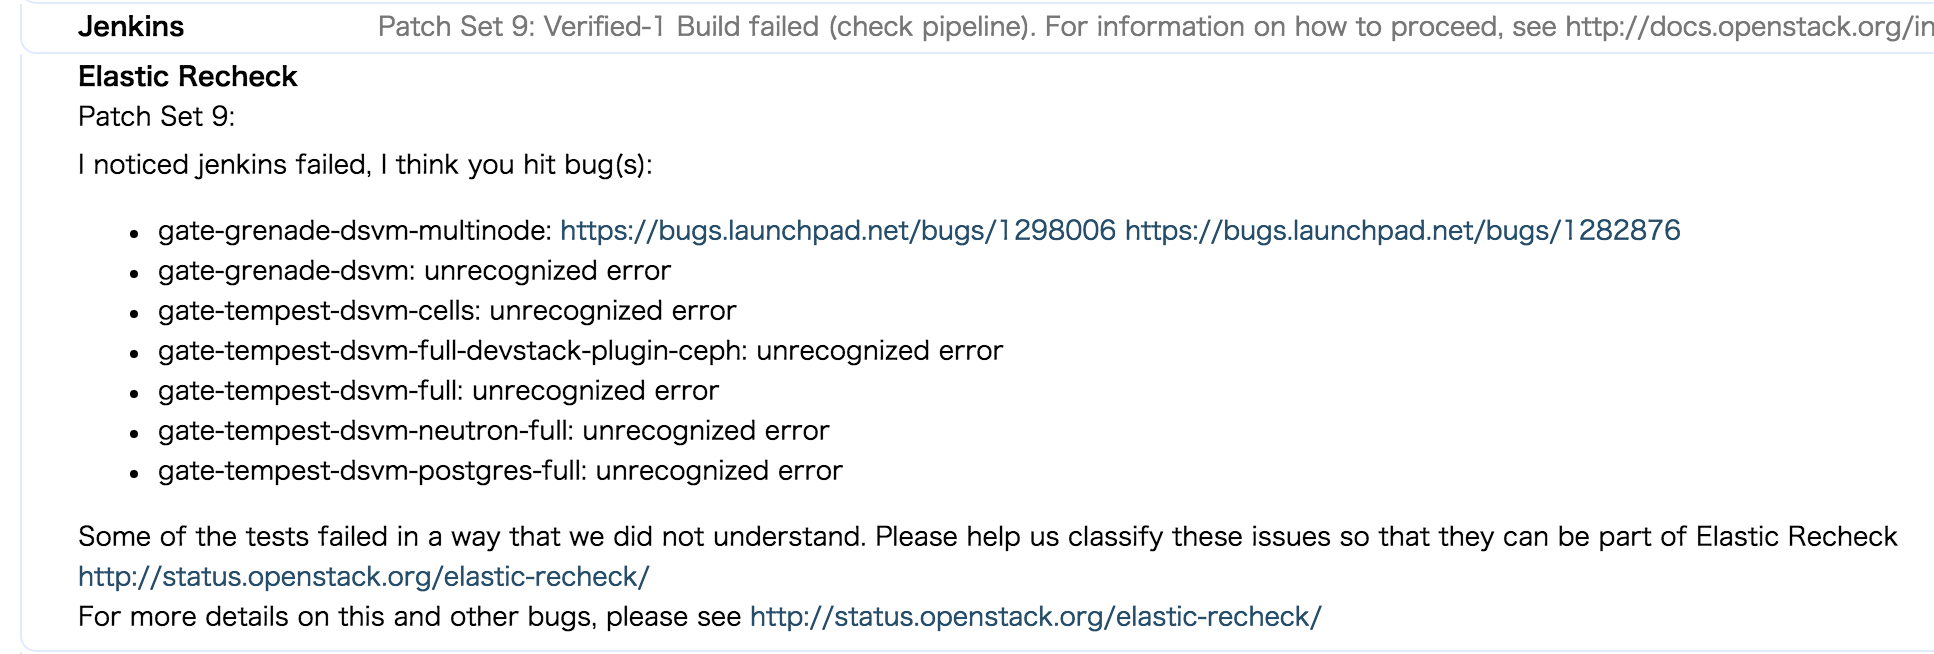
\includegraphics[width=.9\textwidth]{elastic-recheck-sample.png}
  \end{center}
\end{frame}

\begin{frame}
  \frametitle{StackViz}
  個々のCIビルド結果を視覚化するツール
  \begin{itemize}
    \item ソースコード:\href{http://git.openstack.org/cgit/openstack/stackviz}{git.openstack.org/cgit/openstack/stackviz}
  \end{itemize}
  \begin{center}
    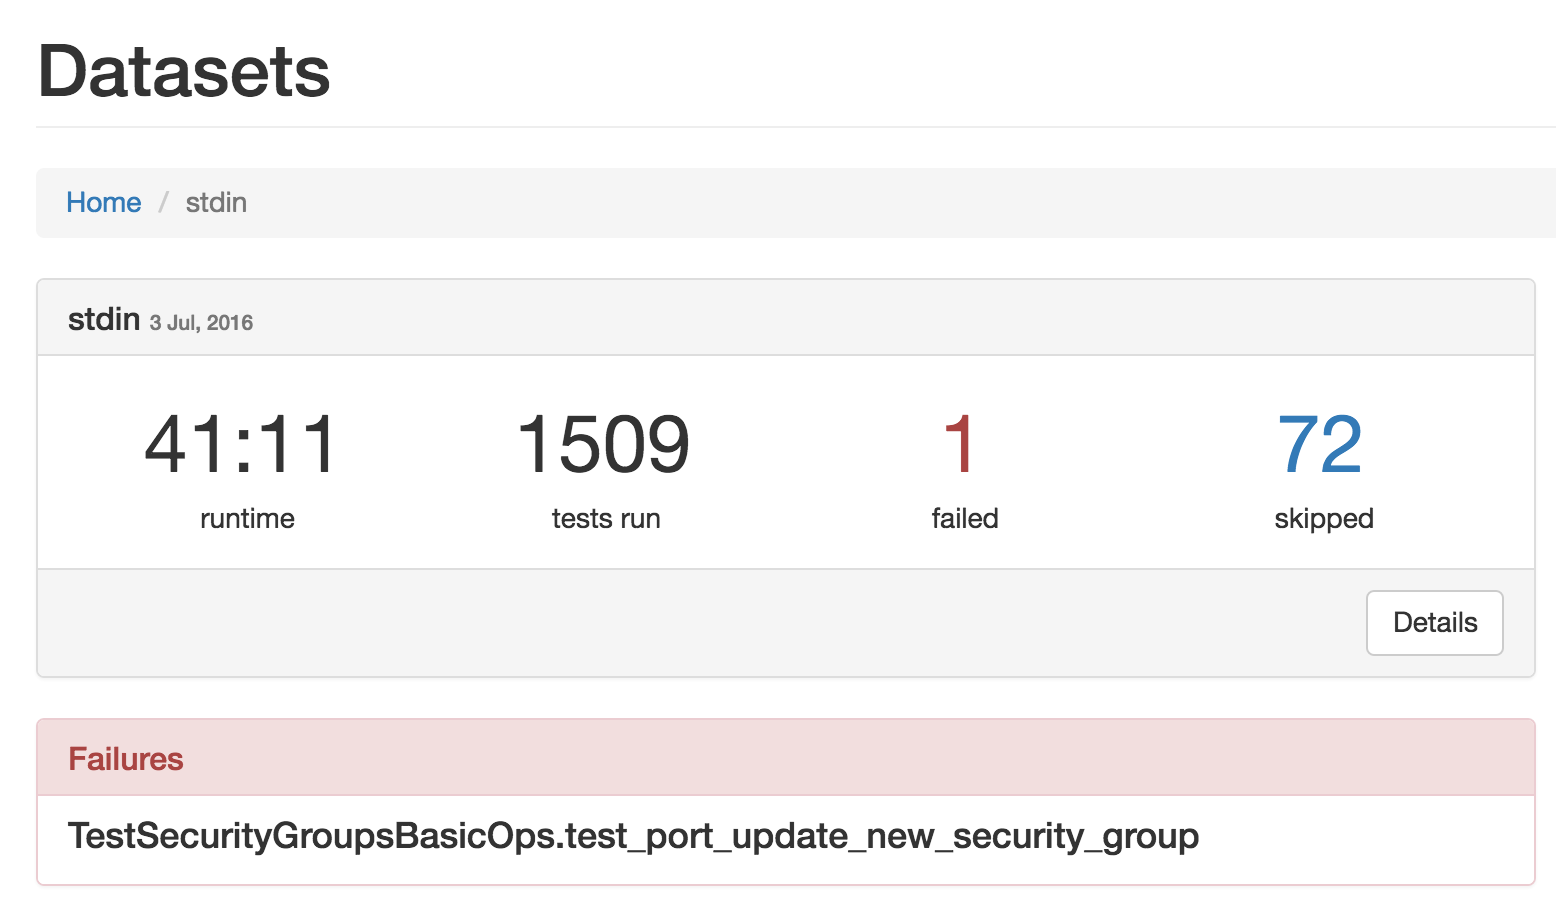
\includegraphics[width=1.3\textheight]{stackviz-sample-top.png}
  \end{center}
\end{frame}

\begin{frame}
  \begin{center}
    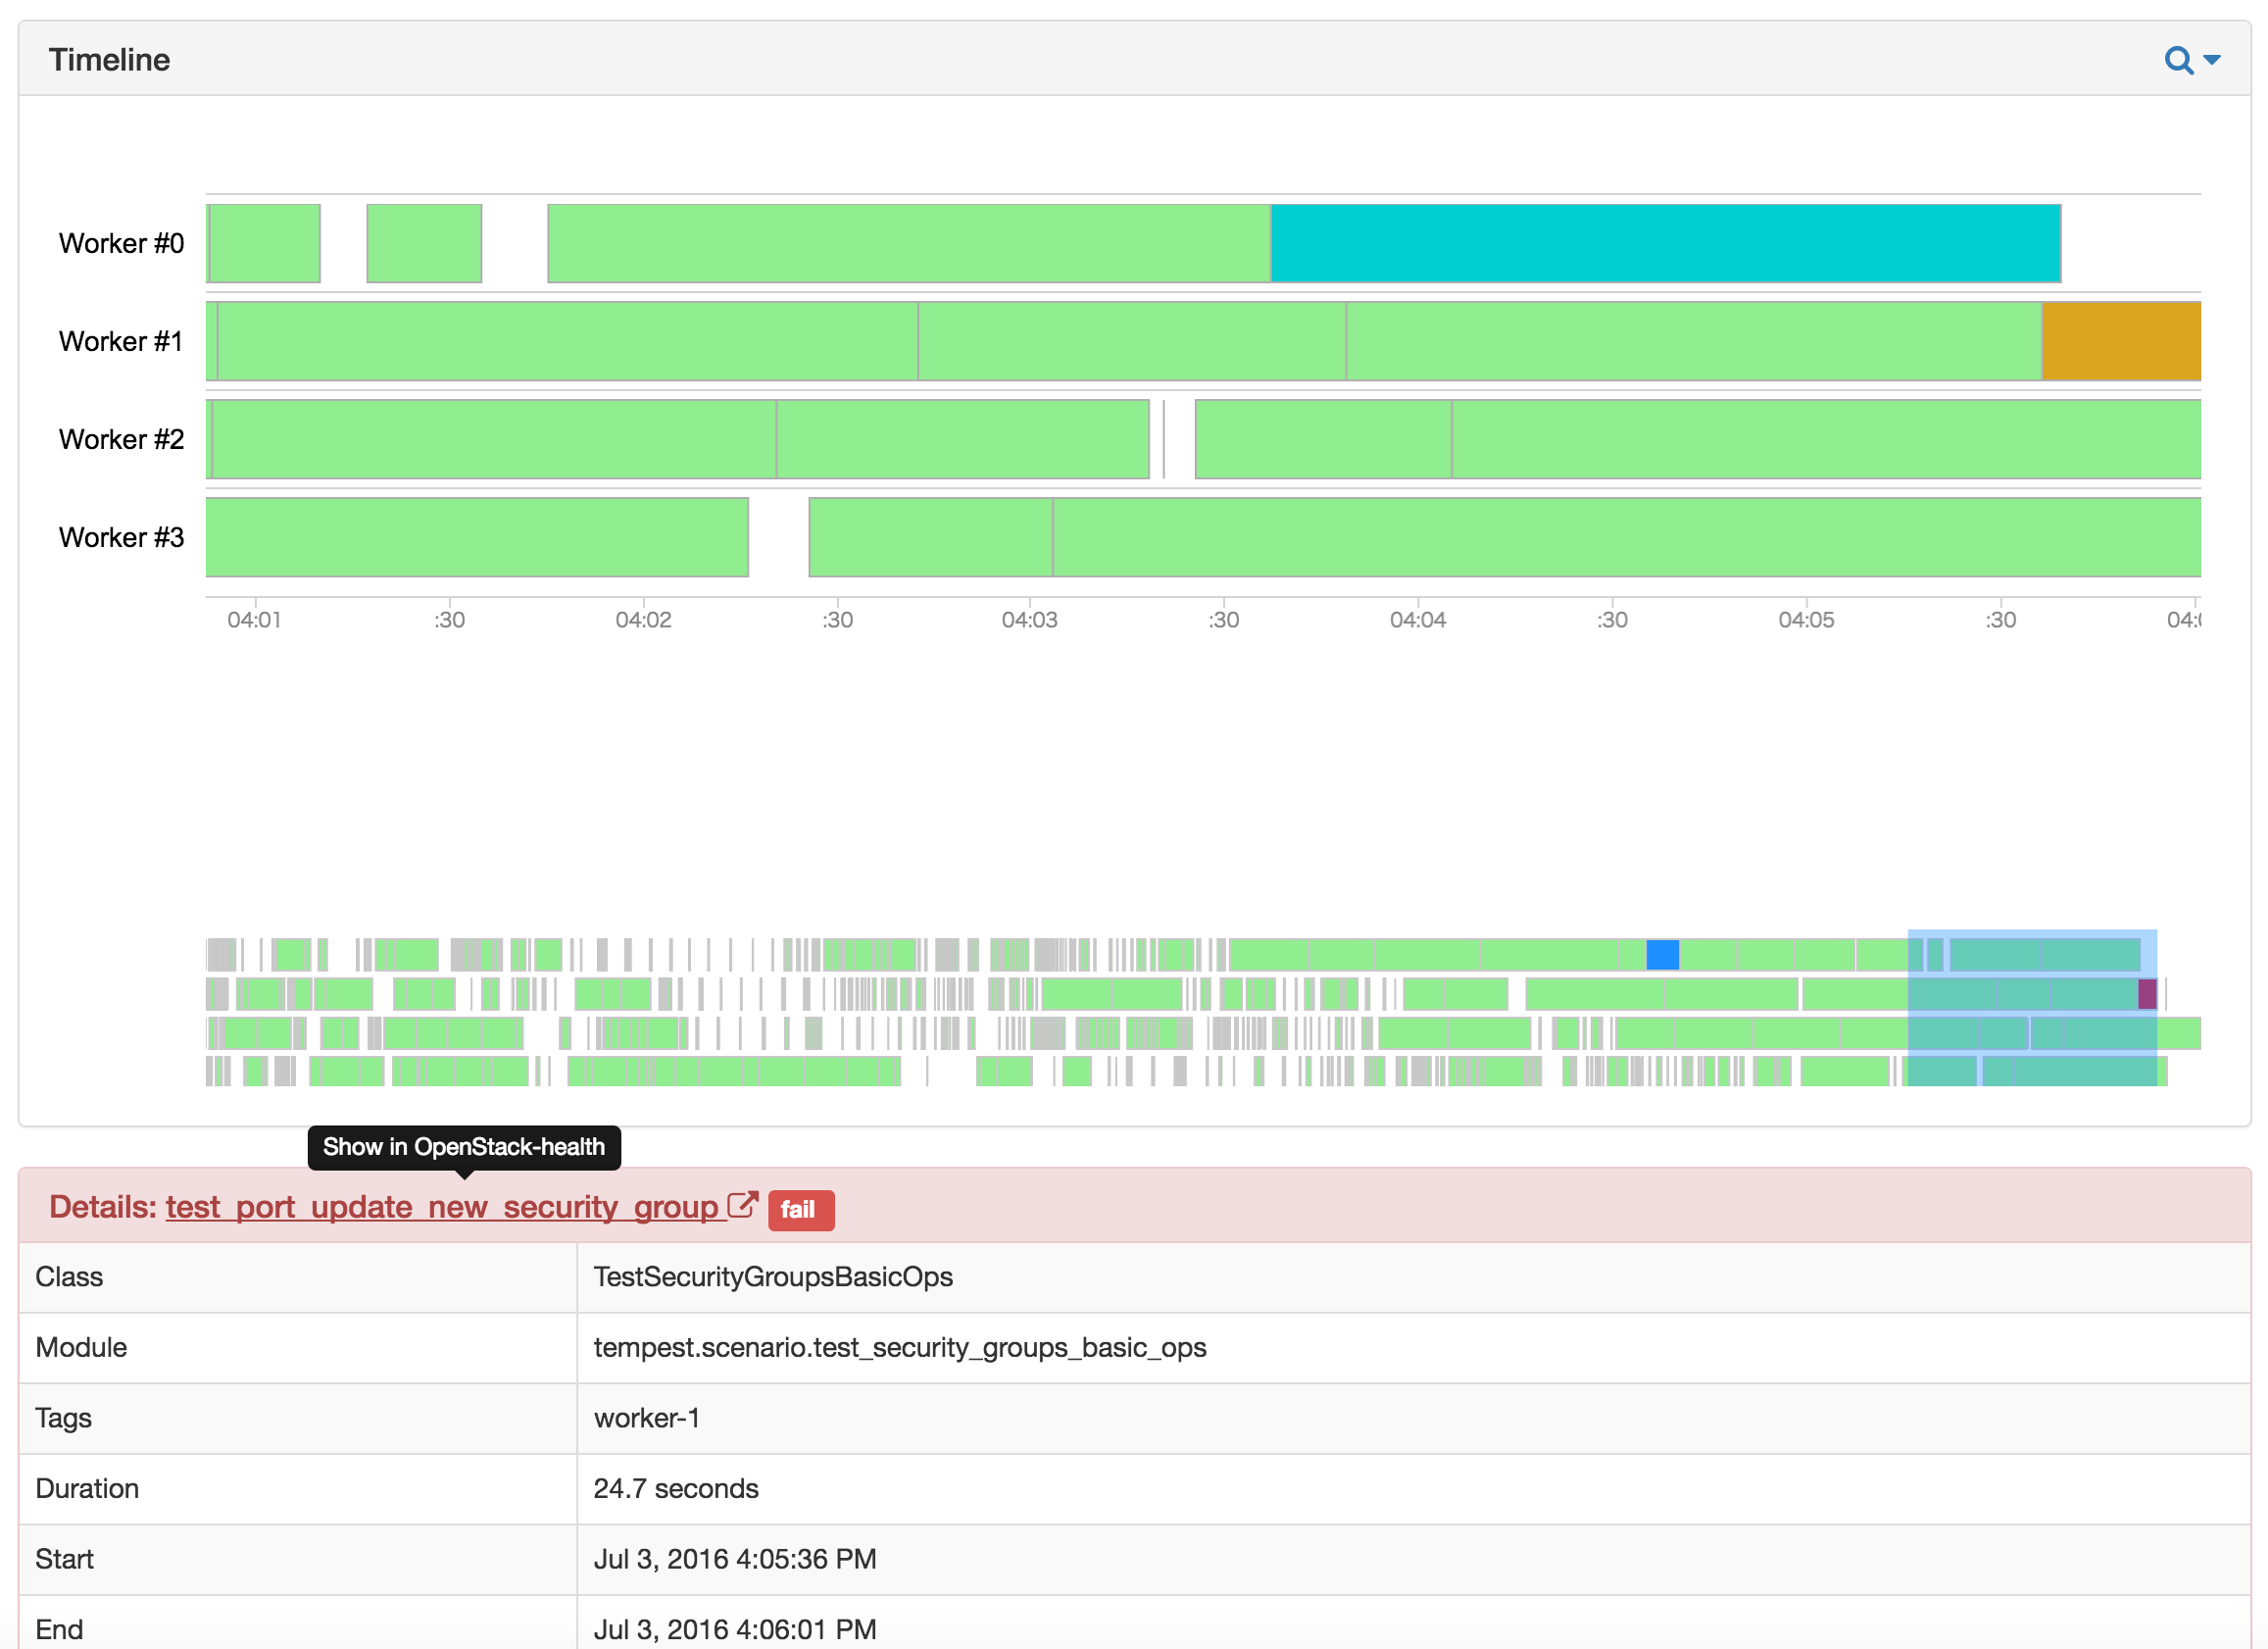
\includegraphics[width=1.3\textheight]{stackviz-sample-timeline.png}
  \end{center}
\end{frame}

\begin{frame}
  \begin{center}
    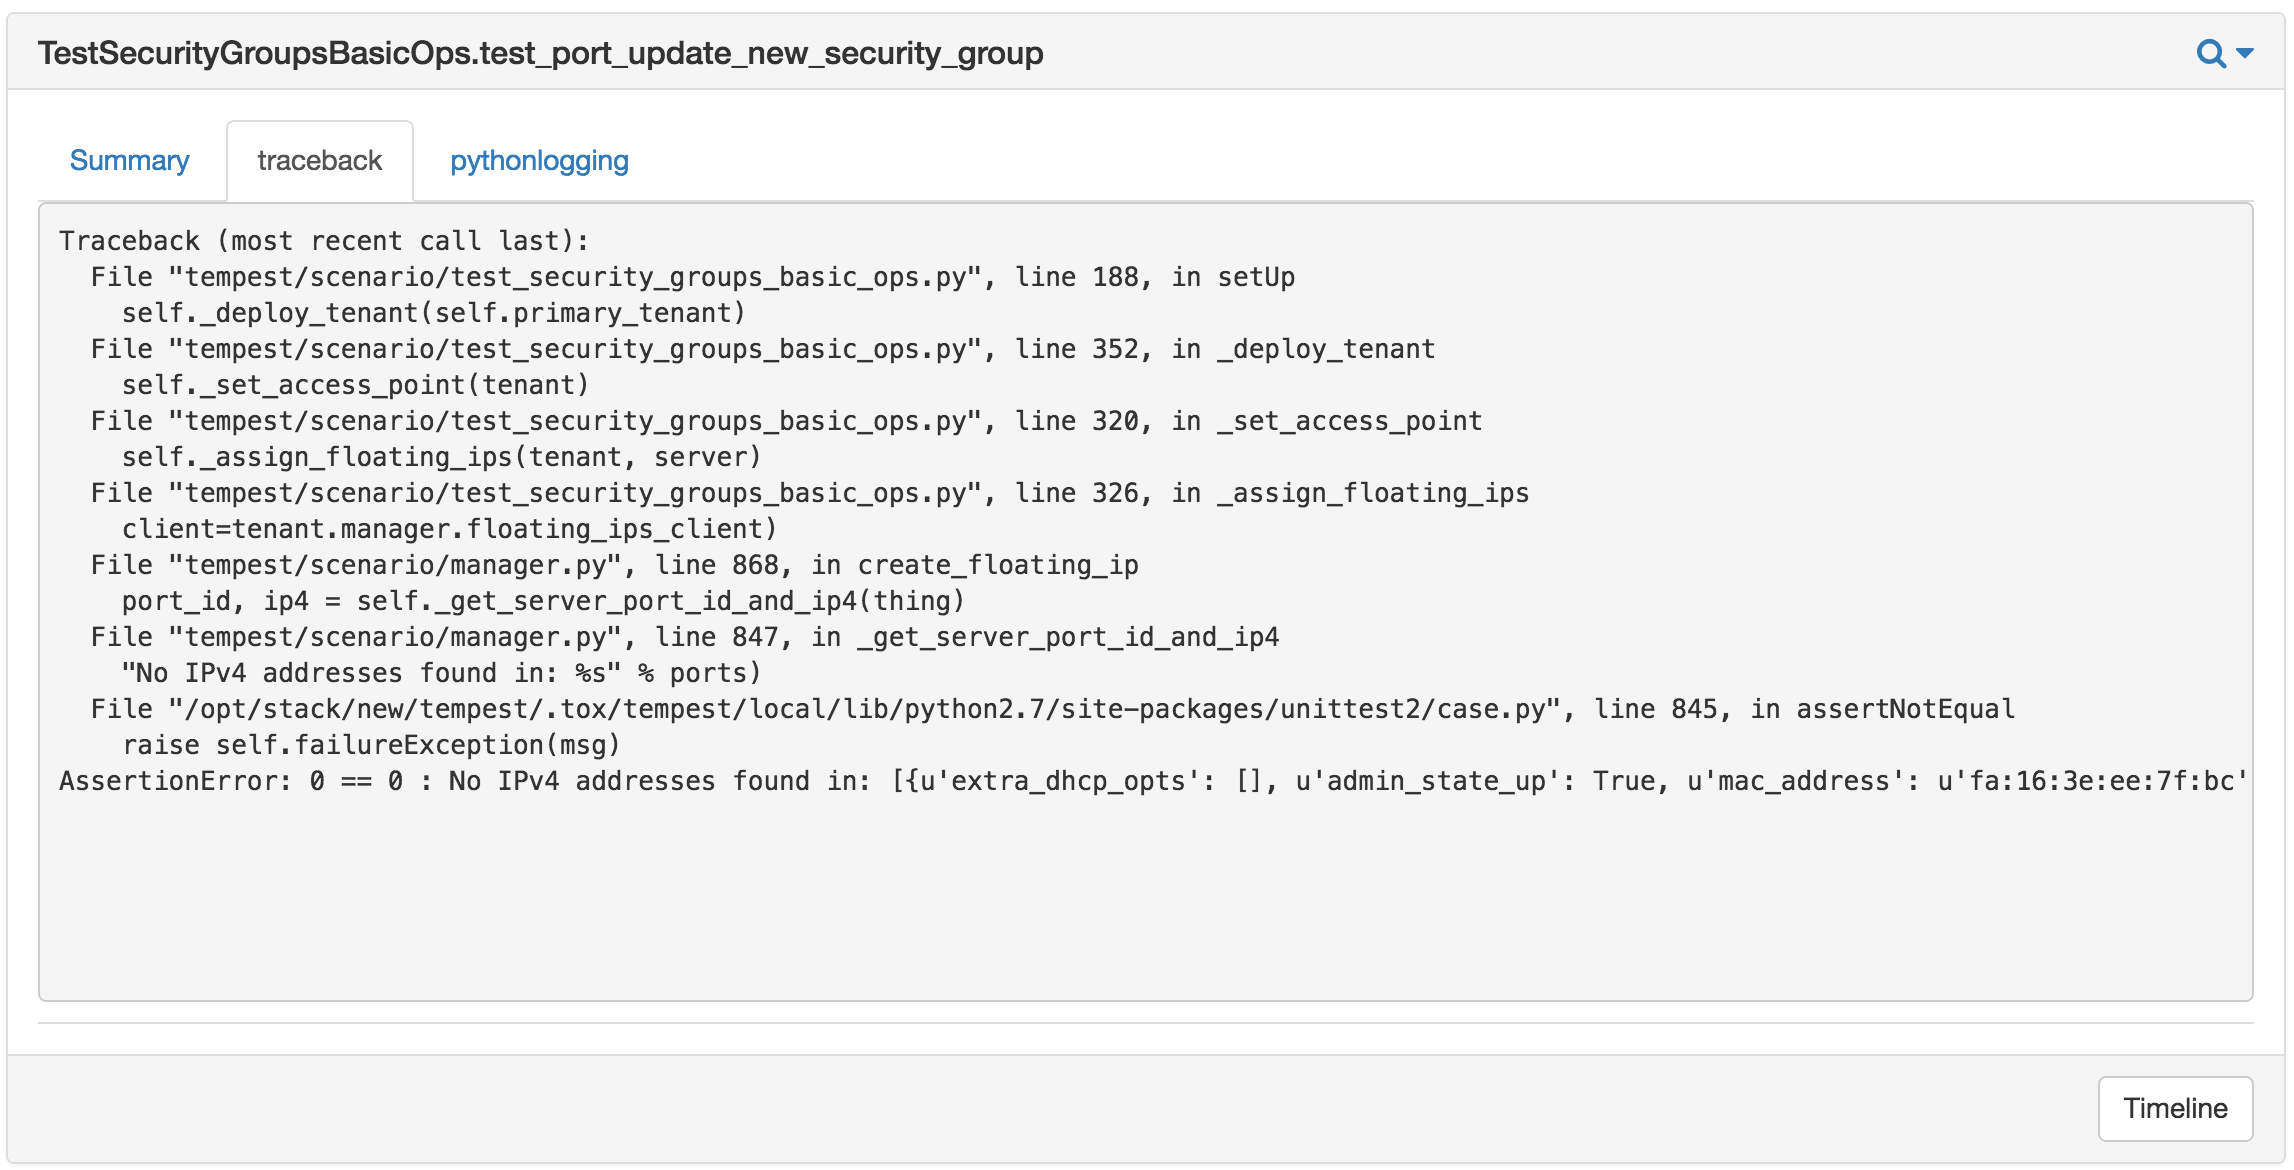
\includegraphics[width=1.3\textheight]{stackviz-sample-traceback.png}
  \end{center}
\end{frame}

\section{Result}
\begin{frame}
  \frametitle{Keep/良かった点}
  \begin{itemize}
    \item 全てのパッチに対してIntegrationテストを実行しており、破滅的な改変などを防いでいる
    \item Job実行結果を俯瞰的に視覚化するにより、パフォーマンス劣化・改善を確認することができた
  \end{itemize}
  \begin{center}
    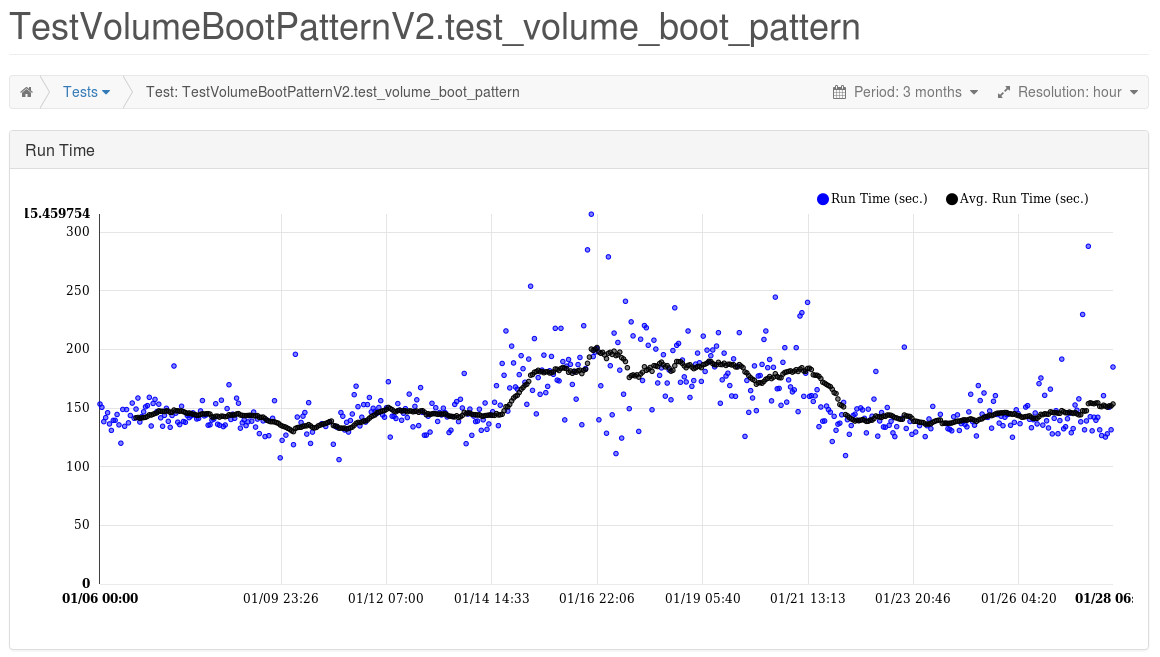
\includegraphics[width=1.1\textheight]{Performance-Issue-o-h.png}
  \end{center}
\end{frame}

\section{Future work/issues}
\begin{frame}
  \frametitle{Problem/改善点}
  \begin{itemize}
    \item 非常に多くの種類のデータ・制限があり、効果的な見せ方が難しい
    \item GateとPeriodicジョブのデータしか保持していない (subunit2sql/openstack-health)
    \item インフラに起因するエラーが対象外 (subunit2sql/openstack-health)
  \end{itemize}
\end{frame}

\begin{frame}
  \frametitle{Try/今後の活動}
  \begin{itemize}
    \item openstack-health改善
    \begin{itemize}
      \item 全てのデータを見られるように
      \item elastic recheckデータの更なる統合
      \item zuulデータの統合
      \item 単体テストカバレッジ推移
    \end{itemize}
    \item 各種UIの改善
    \item 失敗検知の自動化
    \item QAプロジェクトの宣伝
  \end{itemize}
\end{frame}

\section{Summary}
\begin{frame}
  \frametitle{まとめ}
  \begin{itemize}
    \item 活発な開発を維持するため、OpenStackアップストリーム開発ではCIが行われている
    \item CIを支える各種ツールが開発・導入され運用されている
    \begin{itemize}
      \item graphite/grafana
      \item Zuul (Gate)
      \item elastic-recheck
      \item subunit2sql
      \item openstack-health
      \item stackviz, etc.
    \end{itemize}
    \item OpenStack開発を支える、QAに興味がある開発者・支援者募集中!
  \end{itemize}
\end{frame}

\section{Questions}
\begin{frame}
  \frametitle{Questions?}
\end{frame}

\subsection{More Information}
\begin{frame}
\frametitle{Where to get more information}
  \begin{itemize}
    \item openstack-dev ML\: \href{mailto:openstack-dev@lists.openstack.org}{openstack-dev@lists.openstack.org}
    \item \#openstack-qa on Freenode
    \item \url{https://wiki.openstack.org/wiki/QA}
    \item \url{http://git.openstack.org/cgit/openstack/openstack-health/}
    \item \url{http://git.openstack.org/cgit/openstack/stackviz/}
    \item \url{http://git.openstack.org/cgit/openstack-infra/subunit2sql}
    \item \url{http://git.openstack.org/cgit/openstack-infra/elastic-recheck/}
  \end{itemize}
\end{frame}

%\end{CJK*}{UTF8}{hiragino-elcapitan}
%\end{CJK*}{UTF8}{genshingothic}
\end{document}
